\documentclass{article}
\usepackage{fancyhdr}
\usepackage{ctex}
\usepackage{listings}
\usepackage[a4paper, body={18cm,22cm}]{geometry}
\usepackage{amsmath,amssymb,amstext,wasysym,enumerate,graphicx}
\usepackage{float,abstract,booktabs,indentfirst,amsmath}
\usepackage{multirow}
\usepackage{enumitem}
\usepackage{listings}
\usepackage{xcolor}
\usepackage{tabularx}
\setlength{\parindent}{2em}
\renewcommand\arraystretch{1.4}
\setmonofont{DejaVu Sans Mono}
\setCJKmonofont{黑体}
\usepackage[xetex,pagebackref]{hyperref}
% \usepackage{array}
% \usepackage{booktabs}
% \usepackage{url}
% \usepackage{diagbox}
% \usepackage{makecell}
% \usepackage{tikz}
% \usepackage{subcaption}
% \usetikzlibrary{positioning, arrows.meta}
\hypersetup{CJKbookmarks=true,colorlinks=true,citecolor=blue,%
            linkcolor=blue,urlcolor=blue,bookmarksnumbered=true,%
            bookmarksopen=true,breaklinks=true}
\lstset{
    % language = C,
    xleftmargin = 3em,xrightmargin = 3em, aboveskip = 1em,
	backgroundcolor = \color{white}, % 背景色
	basicstyle = \small\ttfamily, % 基本样式 + 小号字体
	rulesepcolor= \color{gray}, % 代码块边框颜色
	breaklines = true, % 代码过长则换行
	numbers = left, % 行号在左侧显示
	numberstyle = \small, % 行号字体
    numbersep = -14pt, 
    keywordstyle=\color{purple}\bfseries, % 关键字颜色
    commentstyle =\color{red!50!green!50!blue!60}, % 注释颜色
    stringstyle = \color{red}, % 字符串颜色
    morekeywords={ASSERT, int64_t, uint32_t},
	frame = shadowbox, % 用(带影子效果)方框框住代码块
	showspaces = false, % 不显示空格
    showstringspaces = false,
	columns = fixed, % 字间距固定
    literate=
        {^+}{{{\color{black}\textbf{+}}\colorbox{green!30}{\phantom{XX}}}}1
        {+\t}{{{\color{black}\textbf{+}}\colorbox{green!30}{\phantom{XX}}}}1,
} 
%--------------------页眉--------------------%
\pagestyle{fancy}
\fancyhead[L]{}
\fancyhead[R]{}
\fancyhead[C]{华东师范大学软件工程学院实验报告}
\fancyfoot[C]{-\thepage-}
\renewcommand{\headrulewidth}{1.5pt}
%--------------------标题--------------------%
\begin{document}

\newcommand{\courseName}{Cloud Computing}
\newcommand{\labName}{鲲鹏云容器实验}
\newcommand{\studentName}{李鹏达}
\newcommand{\studentID}{10225101460}
\newcommand{\grade}{2022级}
\newcommand{\labNo}{No. 2}
\newcommand{\labDate}{2024年12月11日}
\newcommand{\labTime}{第13 - 14周}

\begin{center}
    \LARGE{{\textbf{\heiti 华东师范大学软件工程学院实验报告}}}
    \begin{table}[H]
        \centering
        \begin{tabular}{cp{3cm}<{\centering}ccp{3cm}<{\centering}ccp{3.5cm}<{\centering}}
            实验课程:    & \courseName & \quad & 年\qquad 级: & \grade & \quad & 实验成绩: &  \\
            \cline{2-2} \cline{5-5} \cline{8-8}
            实验名称:    & \labName & \quad & 姓\qquad 名:    & \studentName & \quad & 实验日期: & \labDate
            \\ \cline{2-2} \cline{5-5} \cline{8-8}
            实验编号: &   \labNo   & \quad & 学\qquad 号: & \studentID & \quad & 实验时间: & \labTime\\ \cline{2-2} \cline{5-5} \cline{8-8}
        \end{tabular}
    \end{table}
\end{center}
\rule{\textwidth}{1pt}
%--------------------正文--------------------%
\section{实验内容}
在鲲鹏云容器中完成Docker主机的安装和配置、镜像的搜索和下载、容器生命周期的基本管理、容器网络的管理,并通过Dockerfile来构建nginx镜像,了解Dockerfile镜像构建过程。

\section{实验关键步骤}

\subsection{购买实验资源}

\subsubsection{创建虚拟私有云}

登录华为云,在产品中选择``虚拟私有云 VPC'',创建虚拟私有云。

填写以下基本信息:

\begin{itemize}[noitemsep]
    \item 地域:华北-北京四
    \item 名称:vpc-docker
    \item 可用区:可用区1
    \item 子网名称:subnet-docker
    \item 子网网段:默认
\end{itemize}

\begin{figure}[H]
\centering
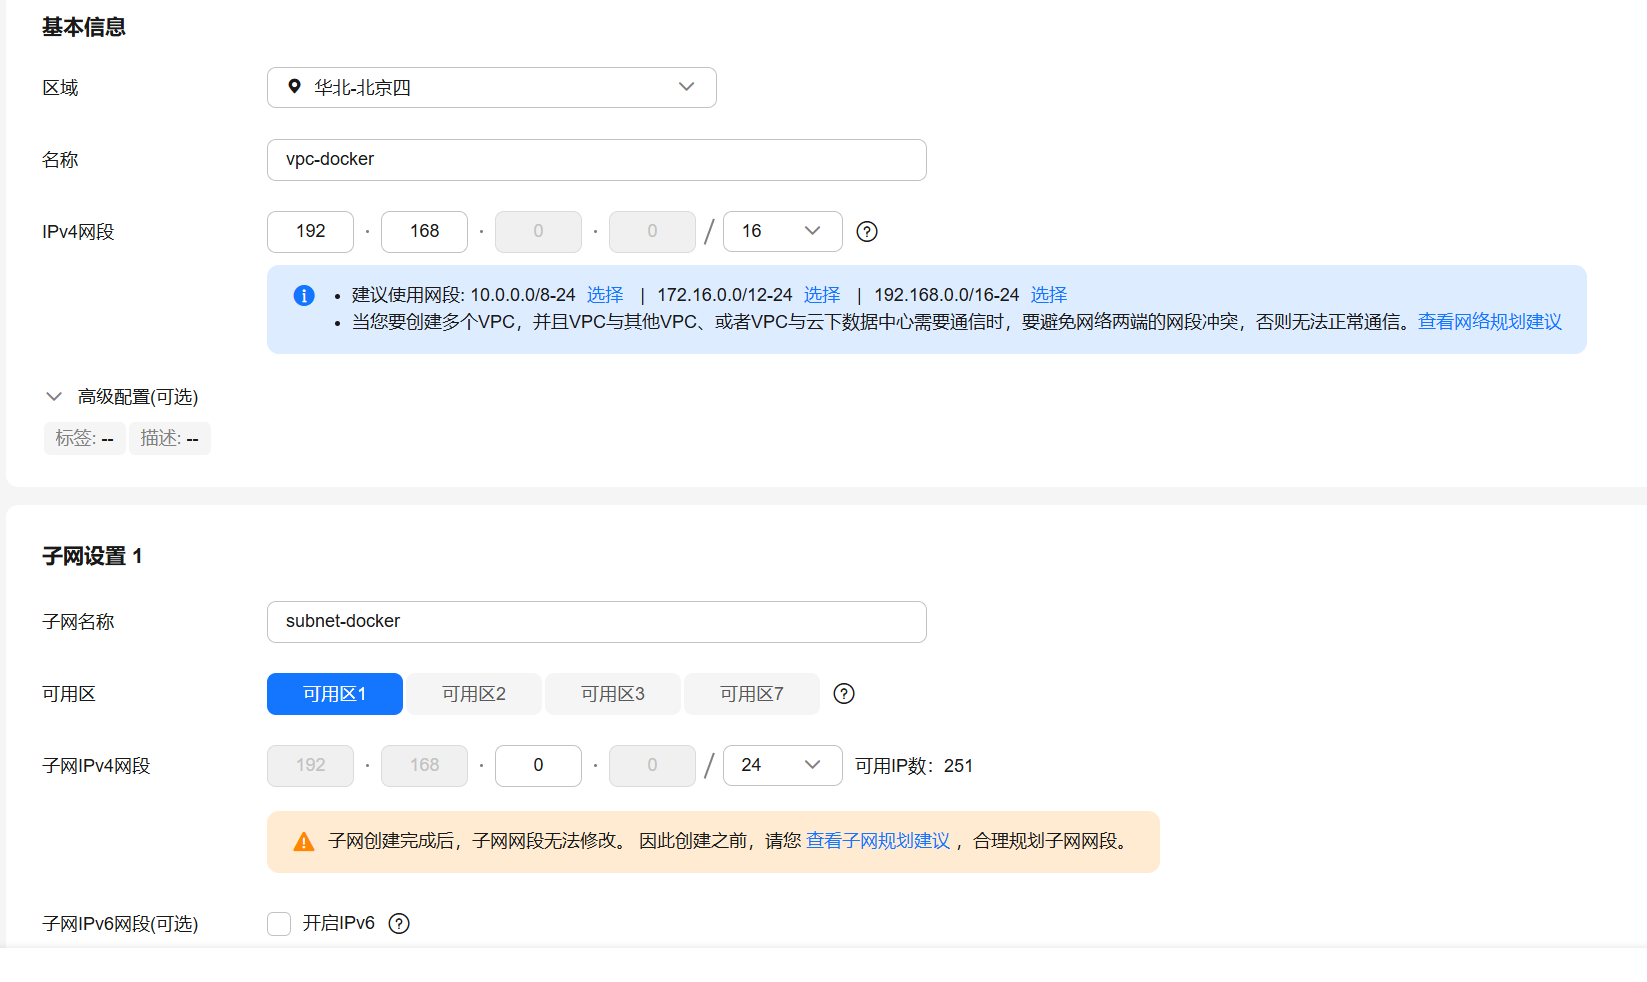
\includegraphics[width=0.5\textwidth]{img/1.1.png}
\caption{创建虚拟私有云}
\end{figure}

\subsubsection{创建并配置安全组}

展开网络控制台左侧列表的访问控制,选择“安全组”,点击“创建安全组”。配置模板选择为“通用Web服务器”,名称设置为“Sys-Webserver”,然后点击“确定”。默认放通22、3389、80、443端口和ICMP协议。

\begin{figure}[H]
\centering
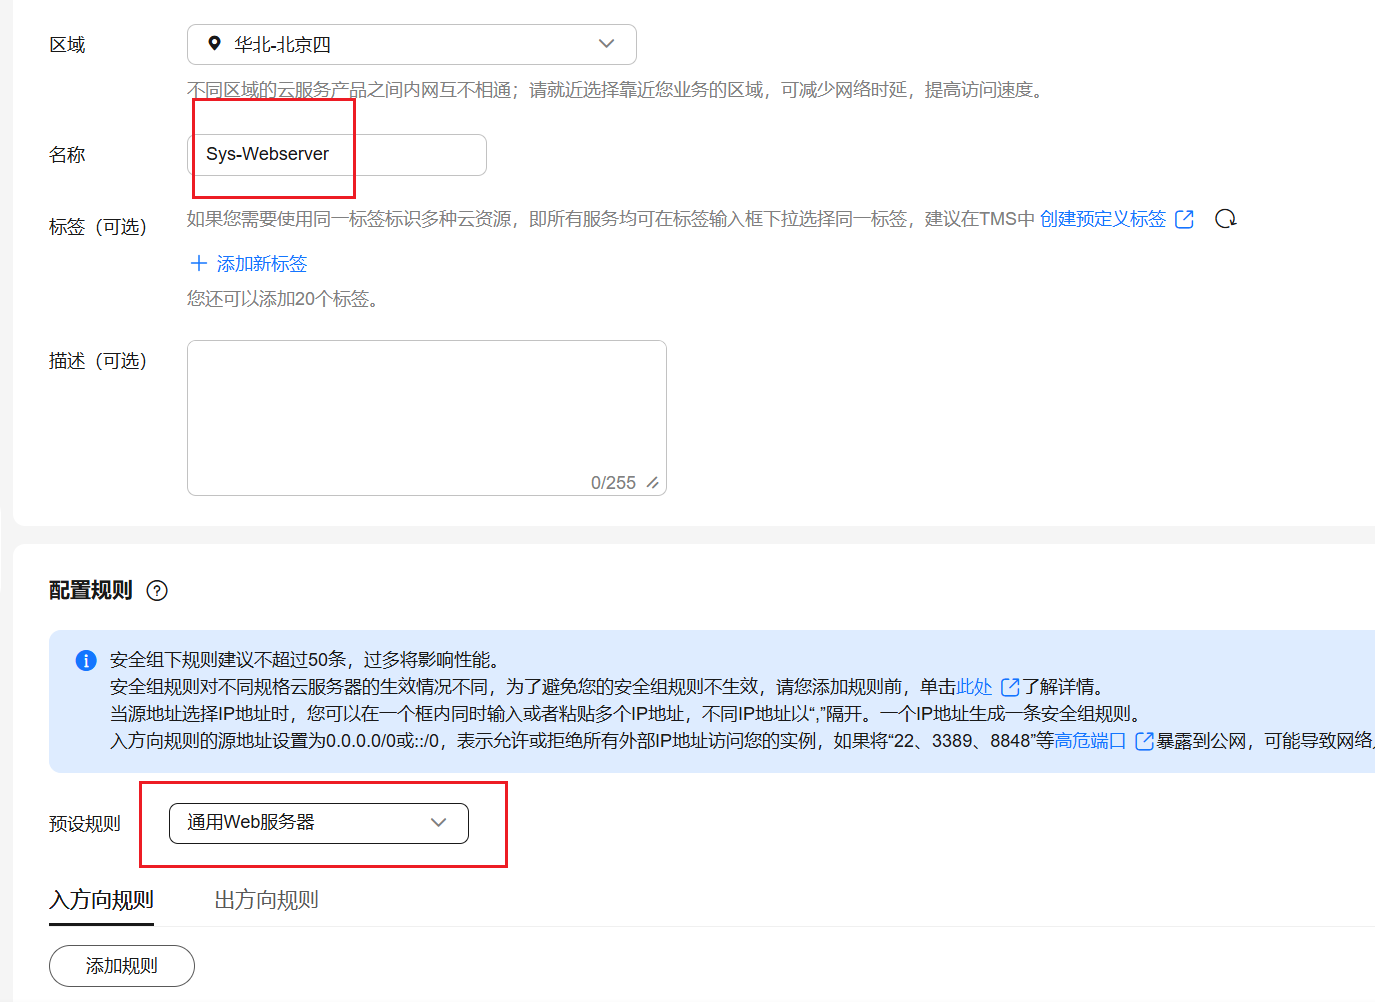
\includegraphics[width=0.9\textwidth]{img/1.2.png}
\caption{创建安全组}
\end{figure}

单击安全组名称“Sys-Webserver”,进入安全组规则配置界面。点击“入方向规则”,为安全起见,将 “全部”放通删除,完成安全组配置。

\begin{figure}[H]
\centering
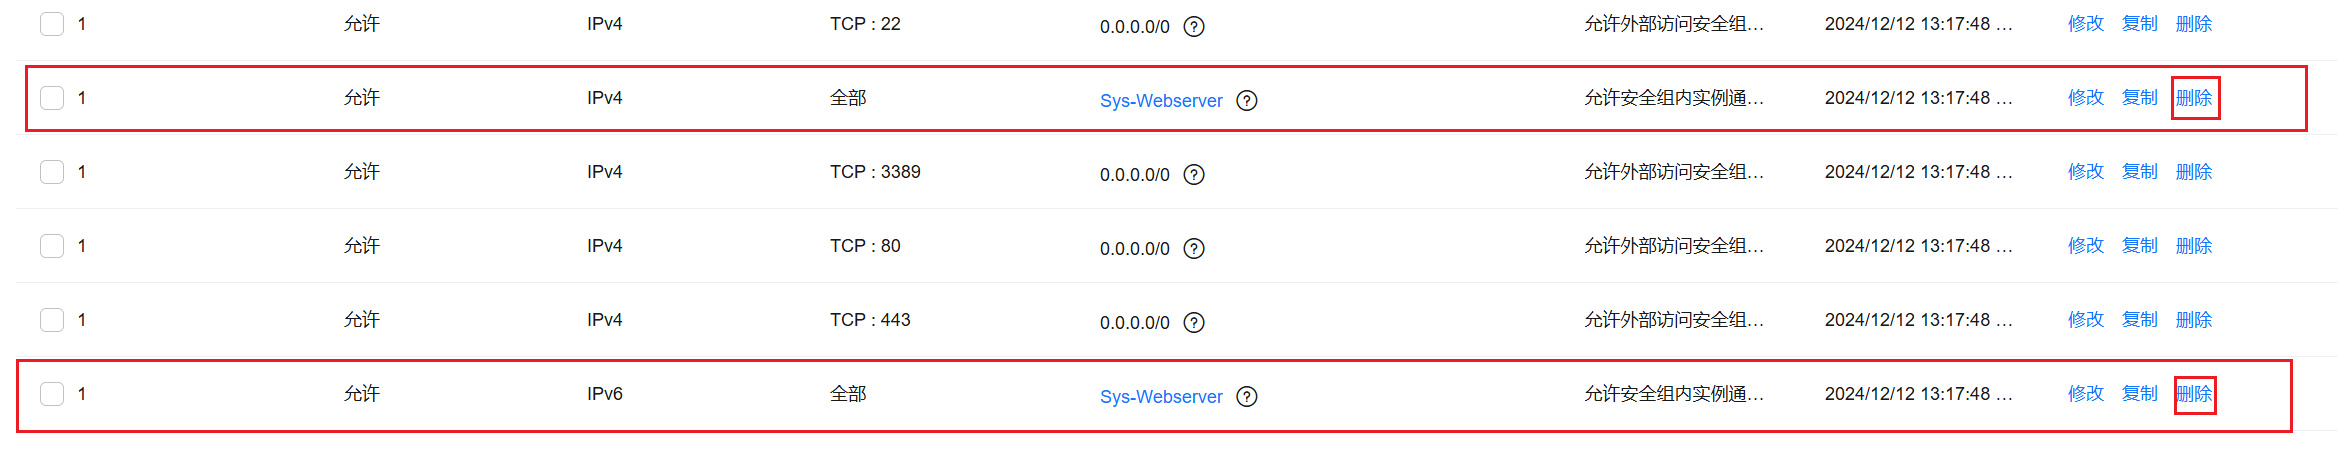
\includegraphics[width=0.9\textwidth]{img/1.3.png}
\caption{配置安全组}
\end{figure}

\subsubsection{购买弹性云服务器}

选择产品\(\to\)基础服务\(\to\)弹性云服务器ECS,然后点击“立即购买”。

填写如下基础配置信息:

\begin{itemize}[noitemsep]
    \item 计费模式:按需计费
    \item 地域:华北-北京四
    \item 可用区:随机分配
    \item CPU架构:鲲鹏计算
    \item 镜像:公共镜像openEuler 20.03 64bit with ARM(40GB)
    \item 系统盘:普通IO/高IO | 40G
    \item 规格:鲲鹏通用计算增强型 | kc1.large.2 | 2vCPUs | 4GB
\end{itemize}

\begin{figure}[H]
\centering
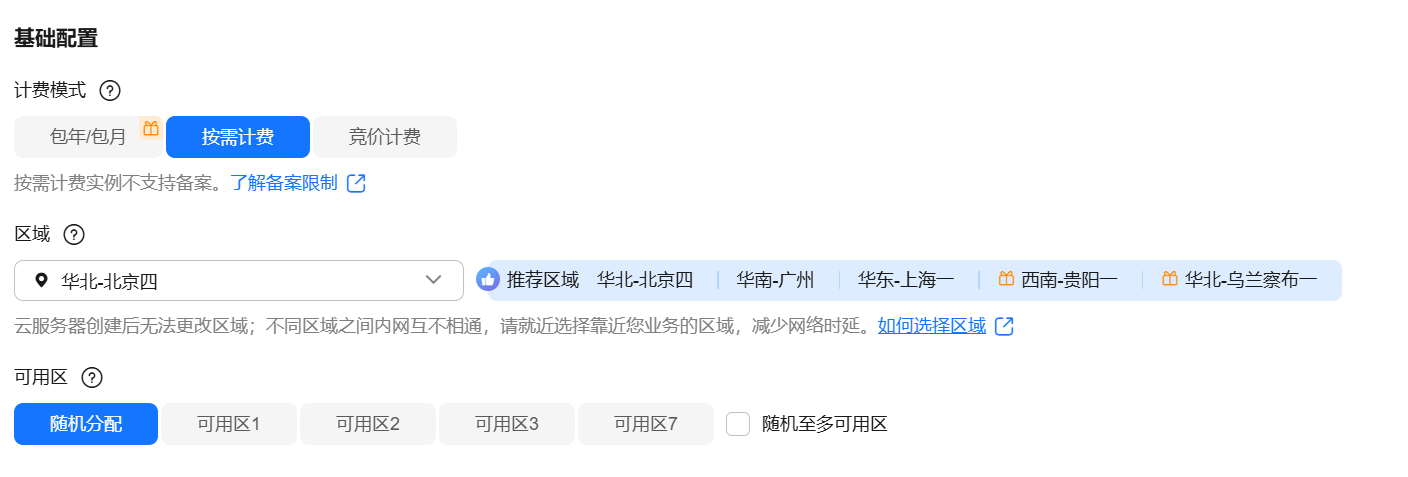
\includegraphics[width=0.8\textwidth]{img/1.4.1.png}
\caption{填写配置信息(1)}
\end{figure}

\begin{figure}[H]
\centering
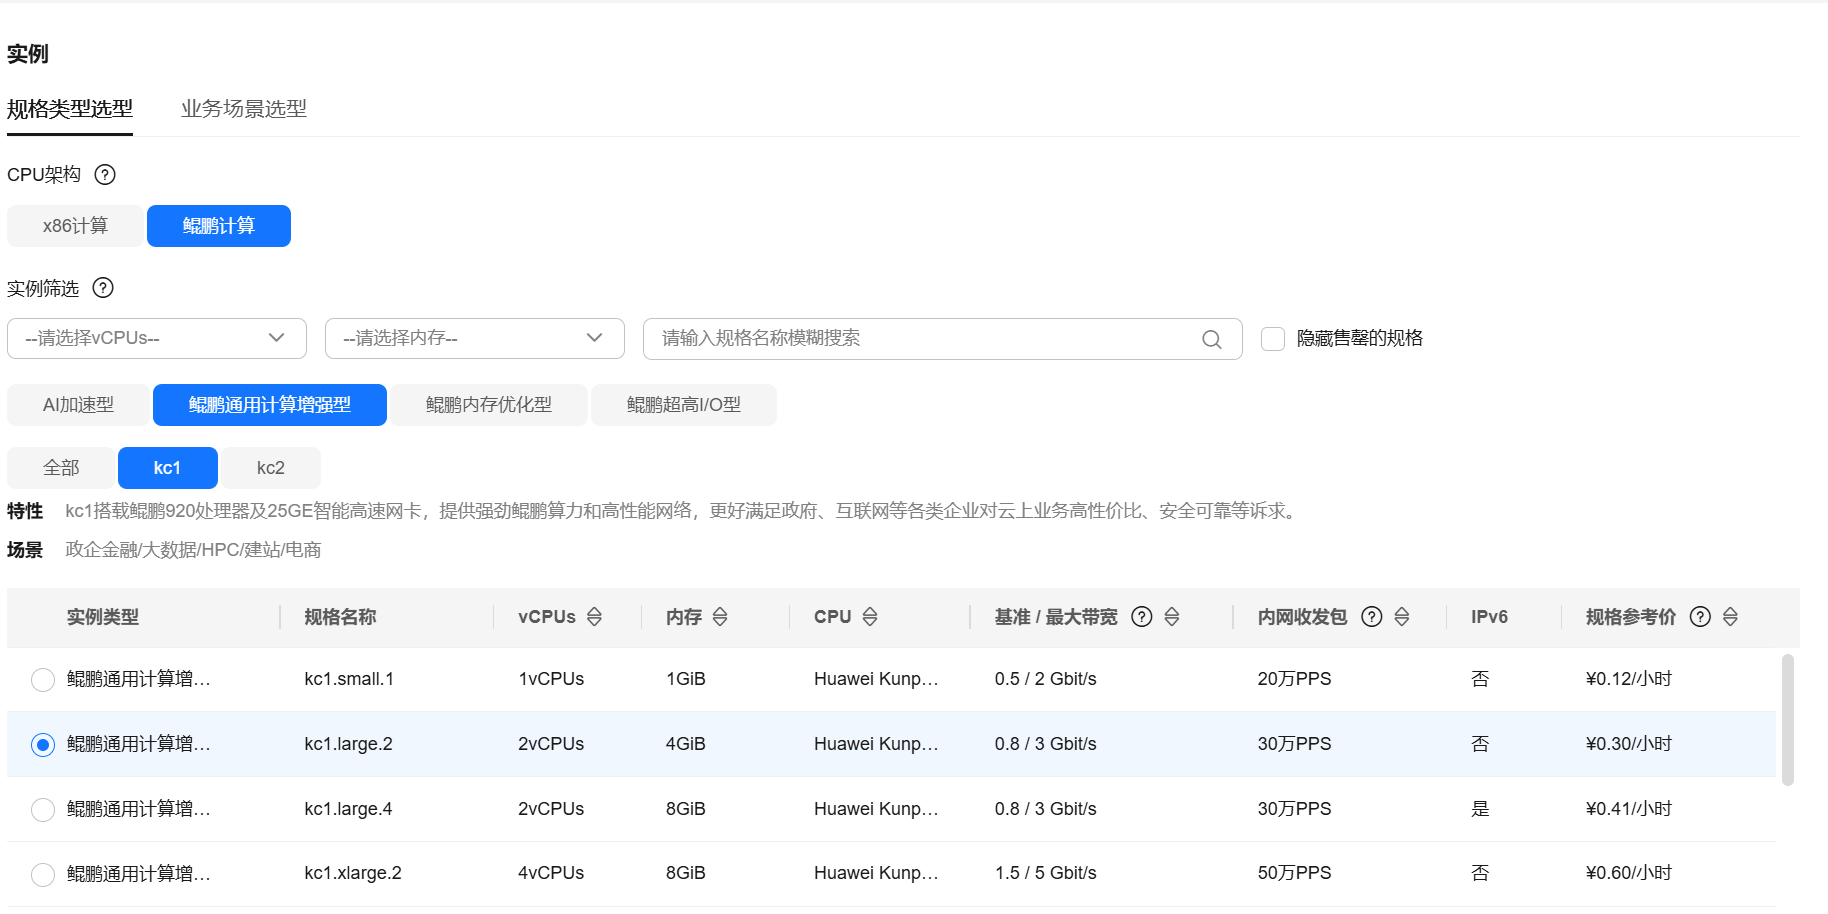
\includegraphics[width=0.8\textwidth]{img/1.4.2.png}
\caption{填写配置信息(2)}
\end{figure}

\begin{figure}[H]
\centering
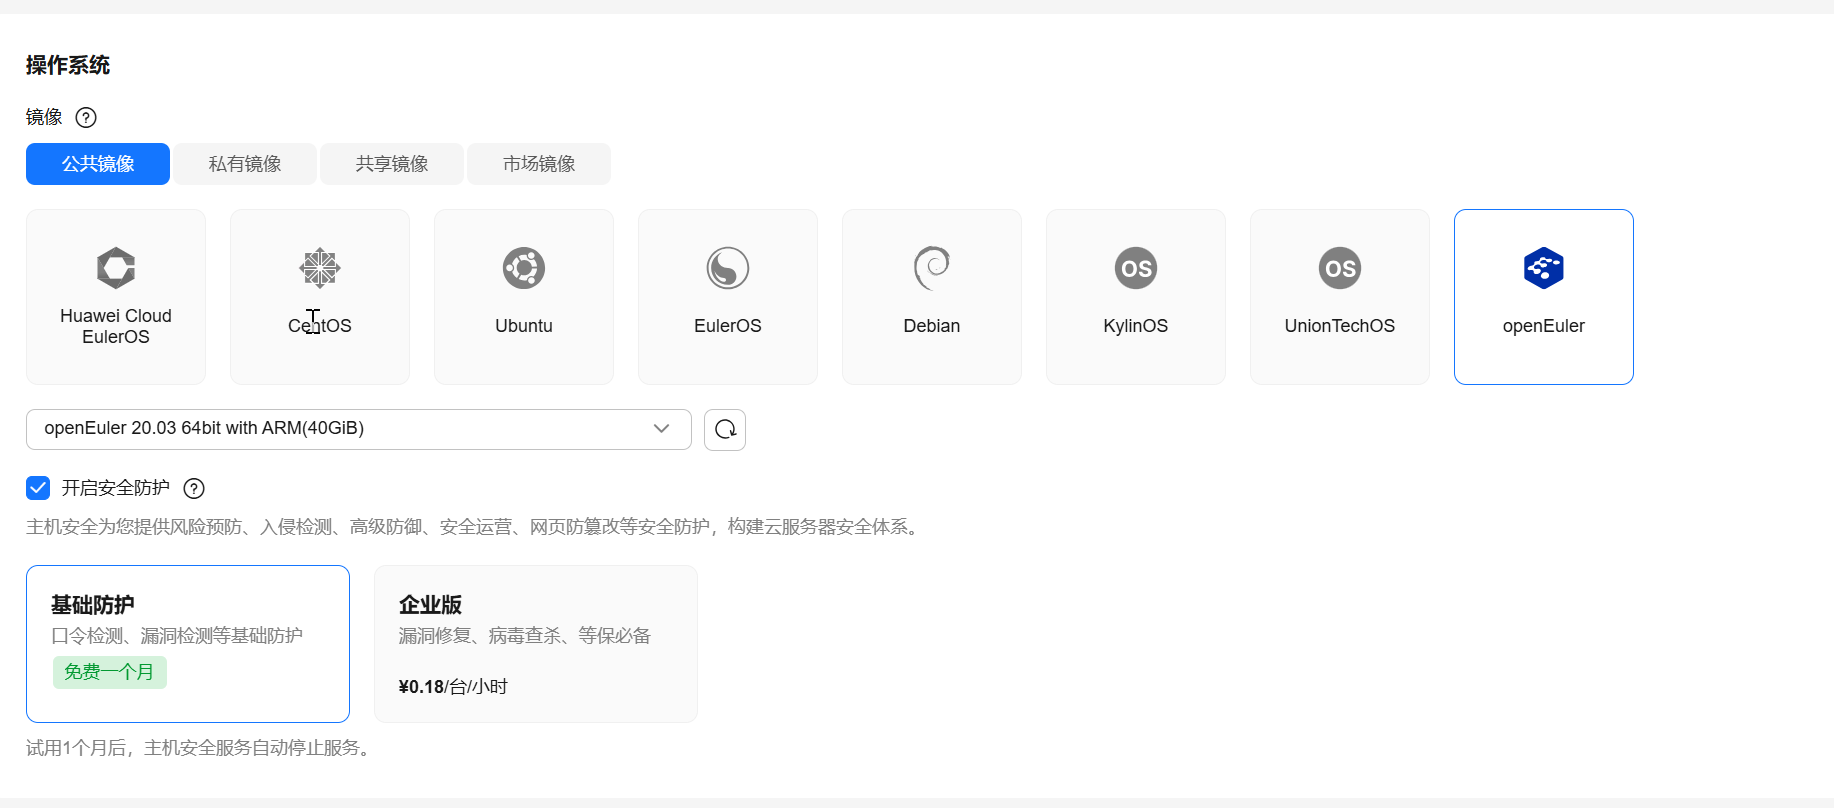
\includegraphics[width=0.8\textwidth]{img/1.4.3.png}
\caption{填写配置信息(3)}
\end{figure}

\begin{figure}[H]
\centering
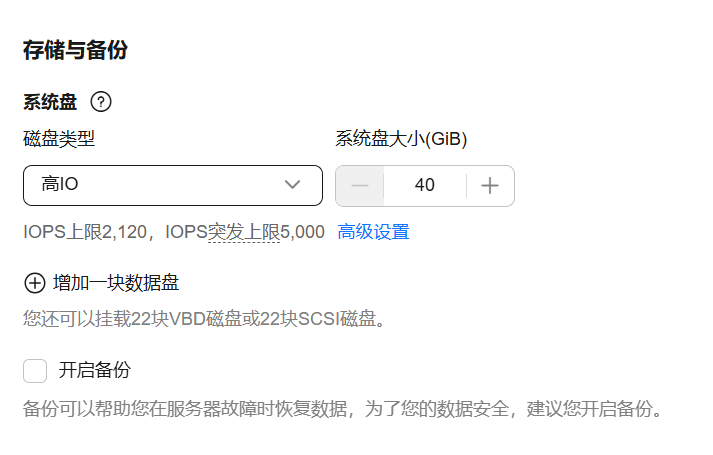
\includegraphics[width=0.6\textwidth]{img/1.4.4.png}
\caption{填写配置信息(4)}
\end{figure}

然后填写如下网络配置信息:

\begin{itemize}[noitemsep]
    \item 网络:选择已创建的网络和子网,如vpc-docker和subnet-docker
    \item 安全组:Sys-Webserver
    \item 弹性公网IP:现在购买
    \item 规格:全动态BGP
    \item 计费方式:按带宽计费
    \item 带宽:5 Mbit/s
\end{itemize}

\begin{figure}[H]
\centering
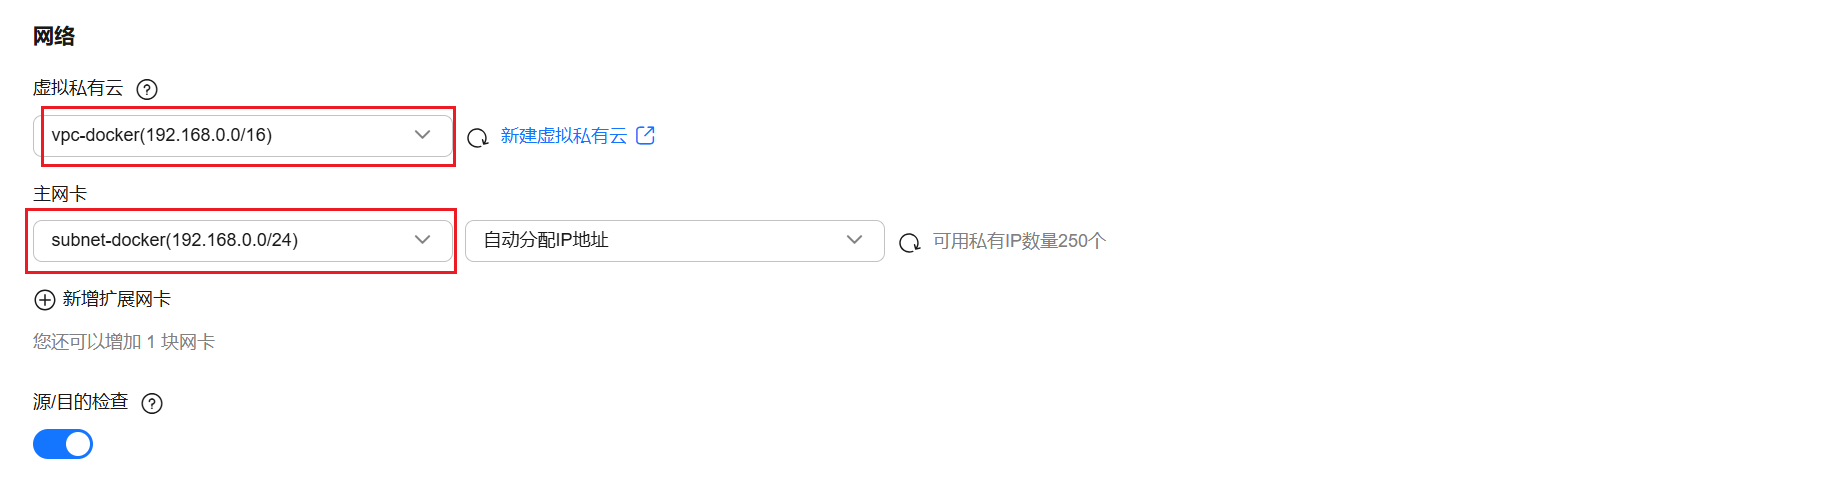
\includegraphics[width=0.8\textwidth]{img/1.4.5.png}
\caption{填写网络配置信息(1)}
\end{figure}

\begin{figure}[H]
\centering
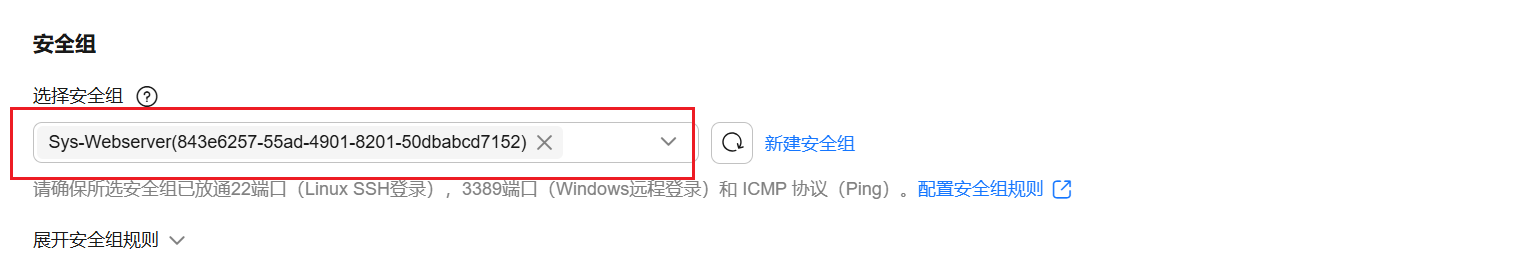
\includegraphics[width=0.8\textwidth]{img/1.4.6.png}
\caption{填写网络配置信息(2)}
\end{figure}

\begin{figure}[H]
\centering
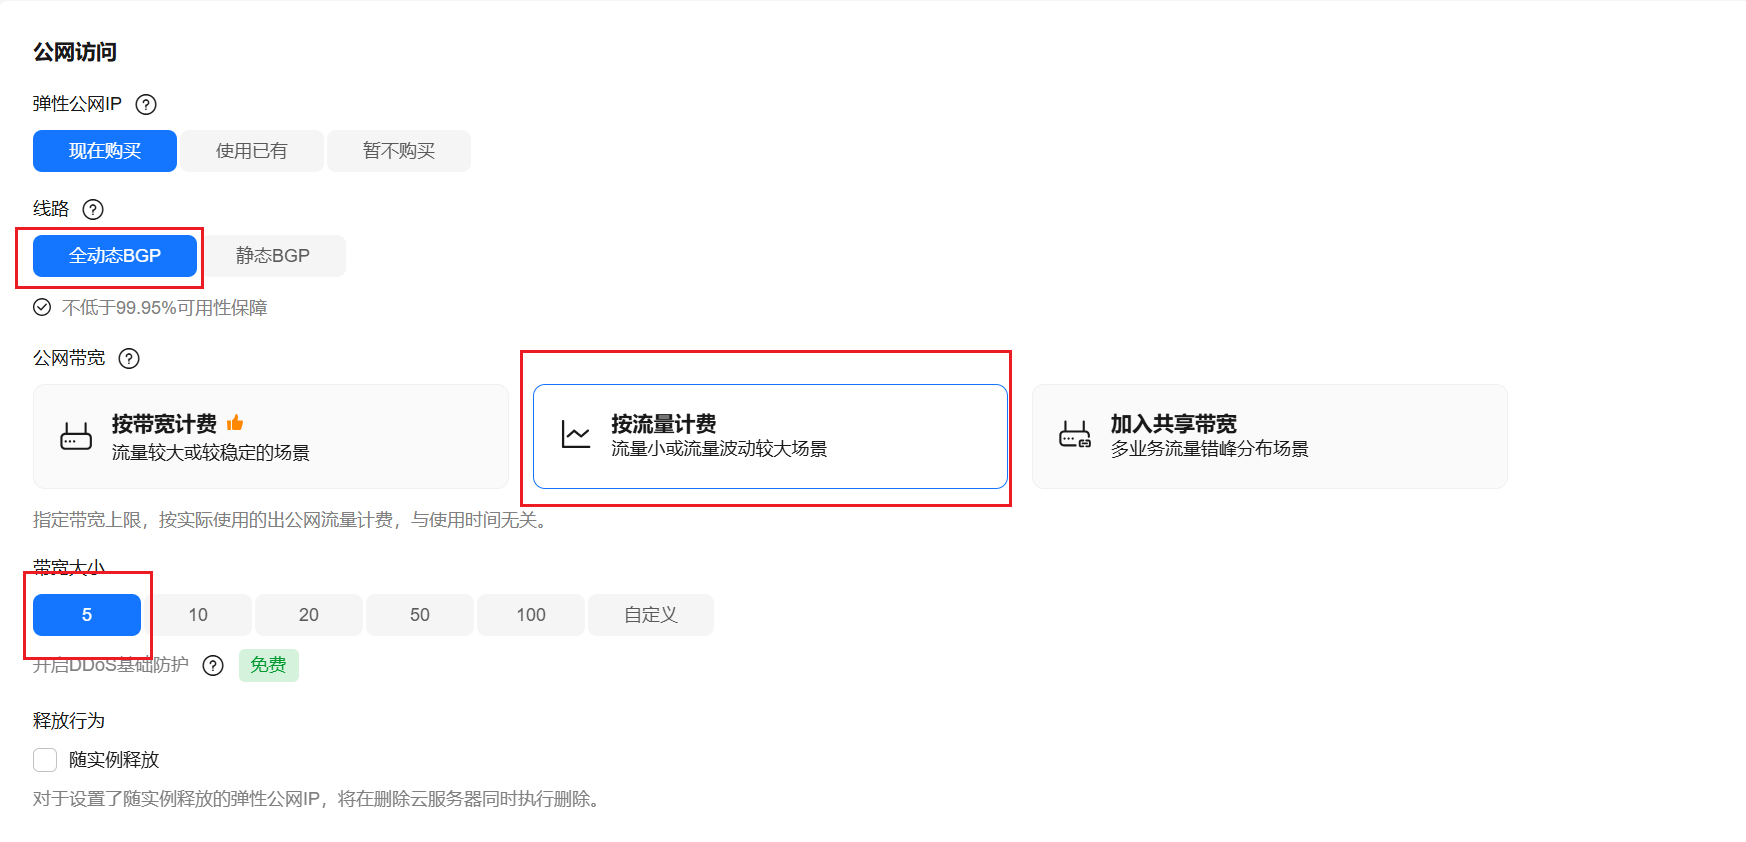
\includegraphics[width=0.8\textwidth]{img/1.4.7.png}
\caption{填写网络配置信息(3)}
\end{figure}

接着,填写如下高级配置信息:


\begin{itemize}[noitemsep]
    \item 云服务器名称:ecs-docker-姓名全拼
    \item 登录凭证:密码
    \item 密码/确认密码:自行设置密码,要求8位以上且包含大小写字母、数字、特殊字符中三种以上字符
\end{itemize}

\begin{figure}[H]
\centering
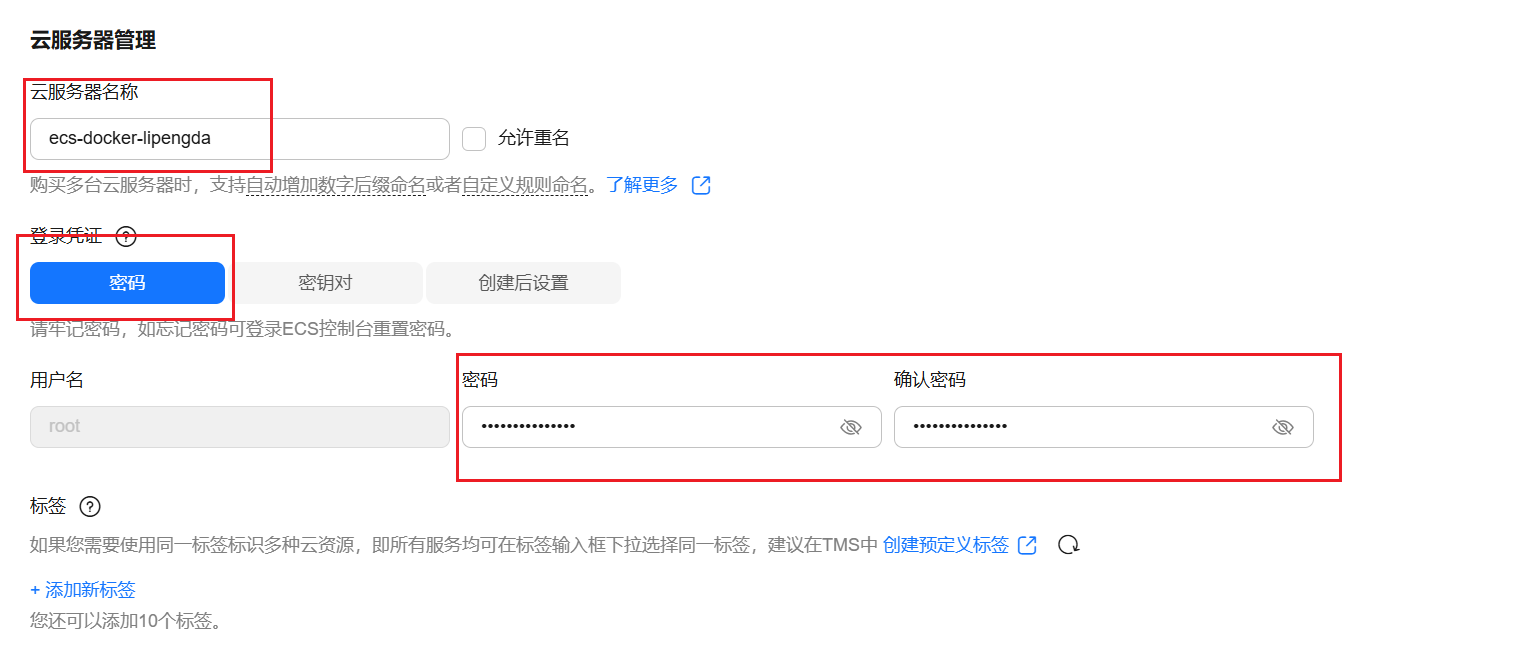
\includegraphics[width=0.9\textwidth]{img/1.4.8.png}
\caption{填写高级配置信息}
\end{figure}

点击创建云服务器,等待创建完成。

创建完成后,可以在控制台中查看创建的云服务器信息。复制弹性公网IP地址,用于后续登录。

\begin{figure}[H]
\centering
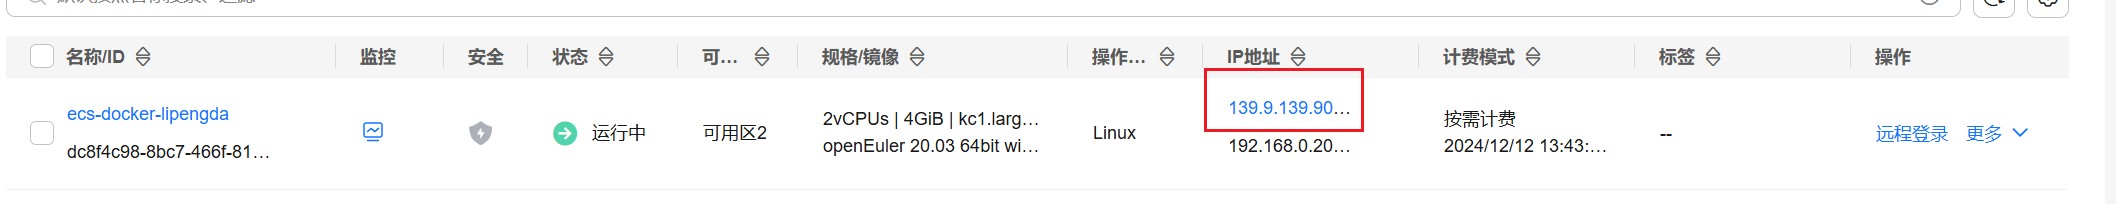
\includegraphics[width=0.9\textwidth]{img/0.1.png}
\caption{查看云服务器信息}
\end{figure}

使用 ssh 登录到创建的云服务器。

\begin{lstlisting}[language=bash]
    ssh root@139.9.139.90
\end{lstlisting}

可以看到出现“welcome to Huawei Cloud Service”,表示登录成功。

\begin{figure}[H]
\centering
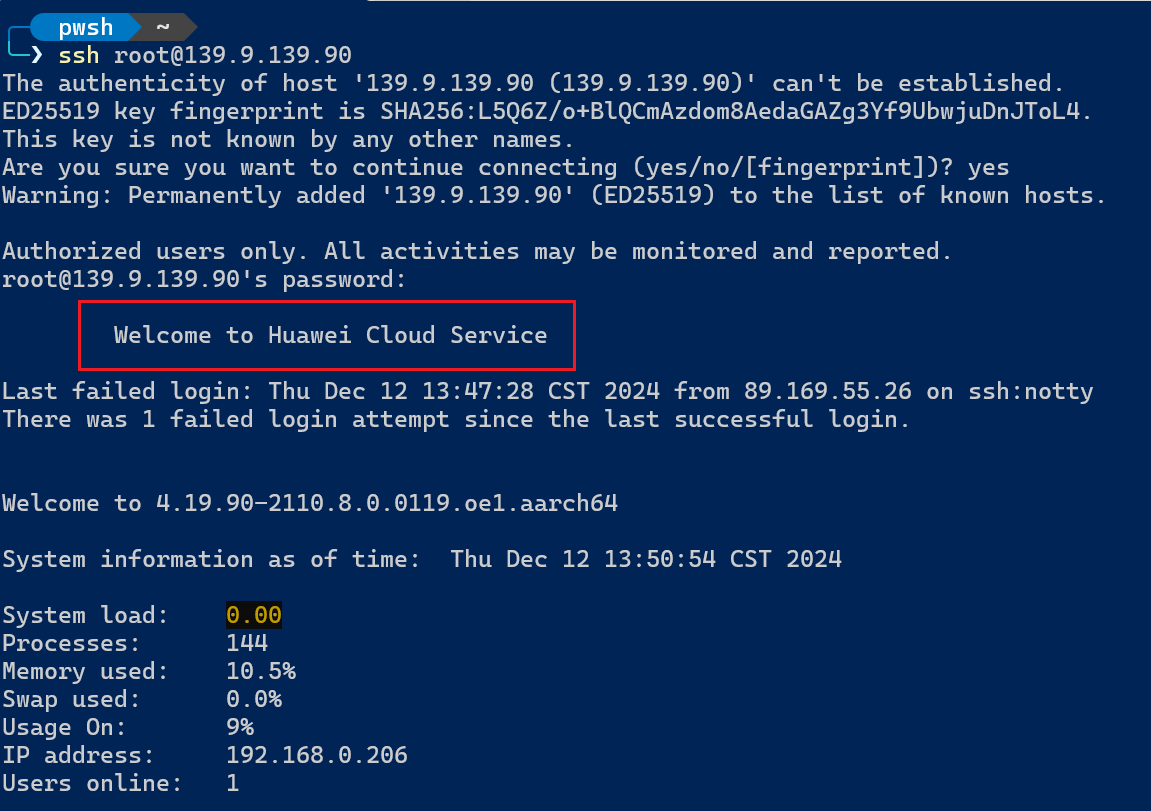
\includegraphics[width=0.9\textwidth]{img/0.2.png}
\caption{登录到云服务器}
\end{figure}

检查内核版本。

\begin{lstlisting}[language=bash]
    uname -r
\end{lstlisting}

\begin{figure}[H]
\centering

\includegraphics[width=0.9\textwidth]{img/1.4.9.png}
\caption{检查内核版本}
\end{figure}

移除旧版本 docker。

\begin{lstlisting}[language=bash]
    yum remove docker docker-client docker-client-latest docker-common docker-latest docker-latest-logrotate docker-logrotate docker-selinux docker-engine-selinux docker-engine
\end{lstlisting}

\begin{figure}[H]
\centering
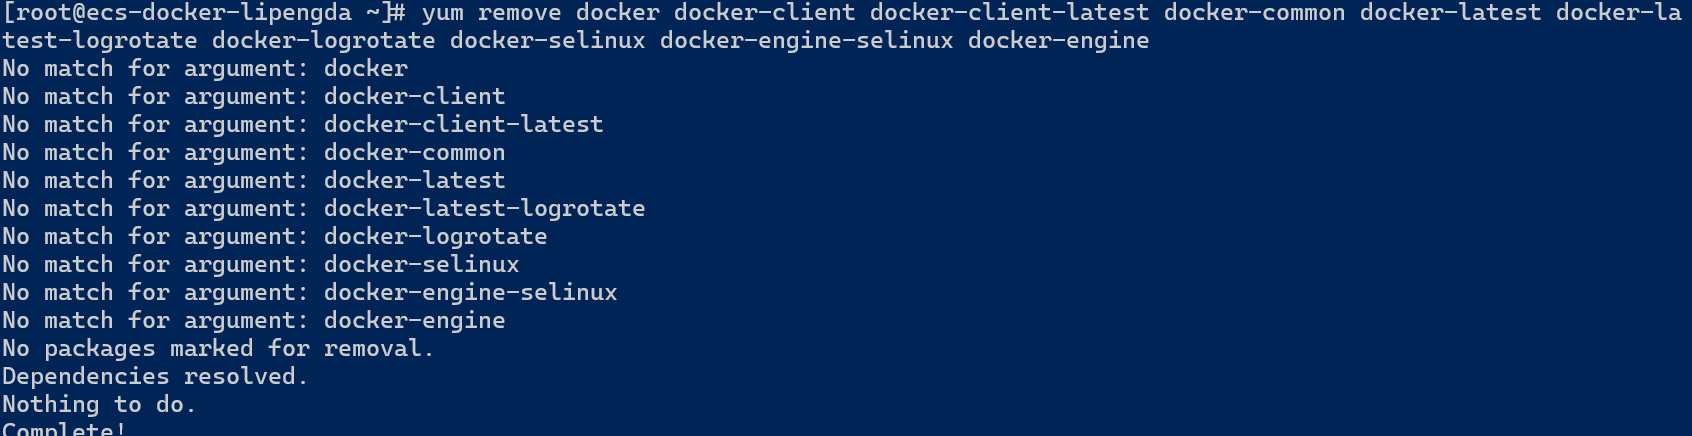
\includegraphics[width=0.9\textwidth]{img/1.4.10.png}
\caption{移除旧版本docker}
\end{figure}

安装Docker依赖工具。

\begin{lstlisting}[language=bash]
    yum install -y device-mapper-persistent-data lvm2
\end{lstlisting}

\begin{figure}[H]
\centering
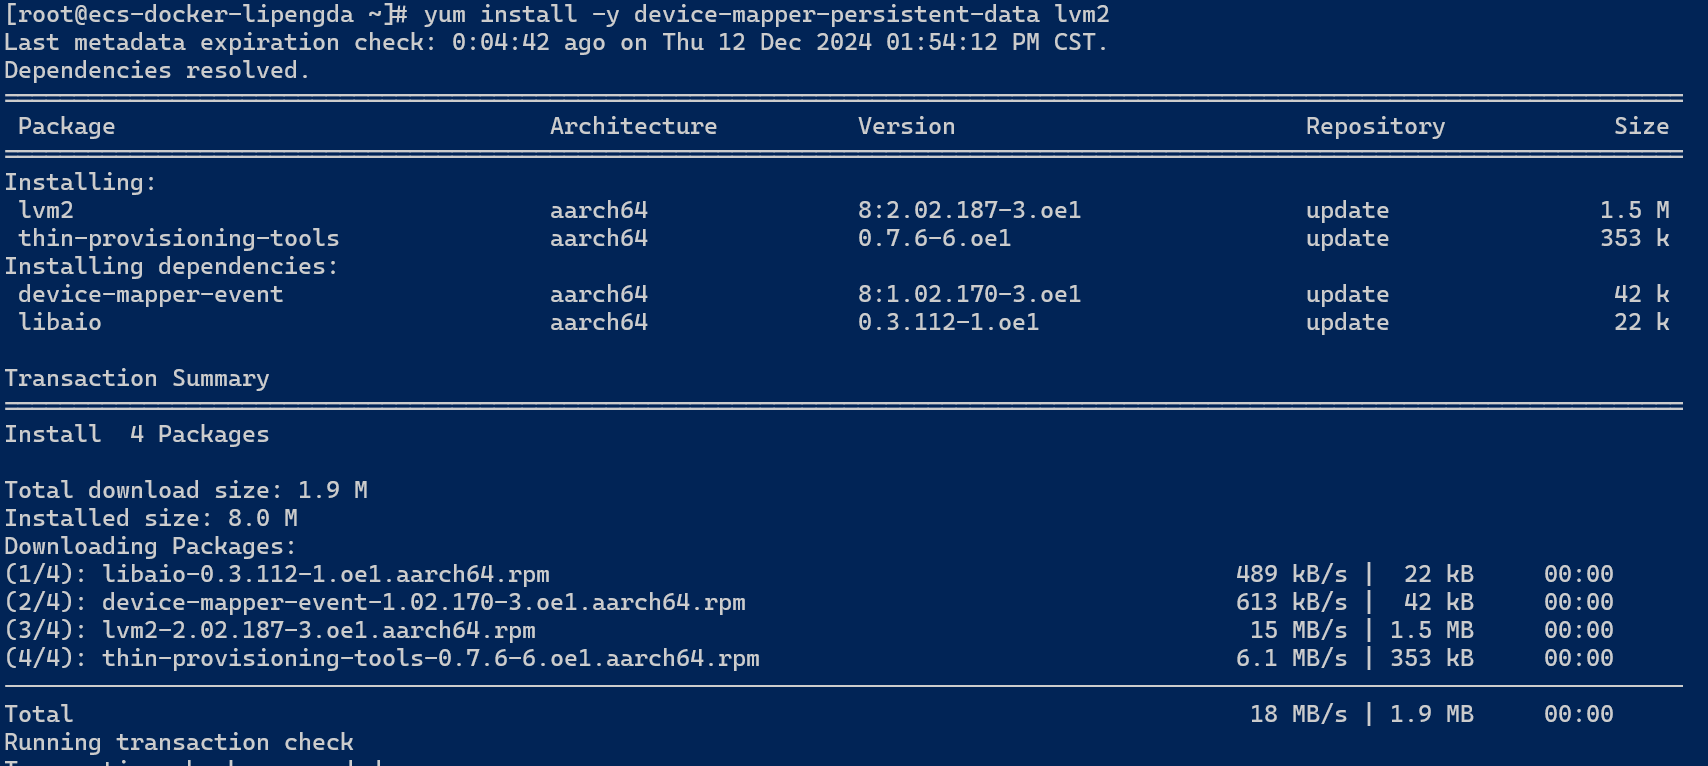
\includegraphics[width=0.9\textwidth]{img/1.4.11.png}
\caption{安装Docker依赖工具}
\end{figure}

\subsection{Docker的安装和配置}

\subsubsection{安装Docker}

安装 Docker。

\begin{lstlisting}[language=bash]
    yum -y install docker --nogpgcheck
\end{lstlisting}

\begin{figure}[H]
\centering
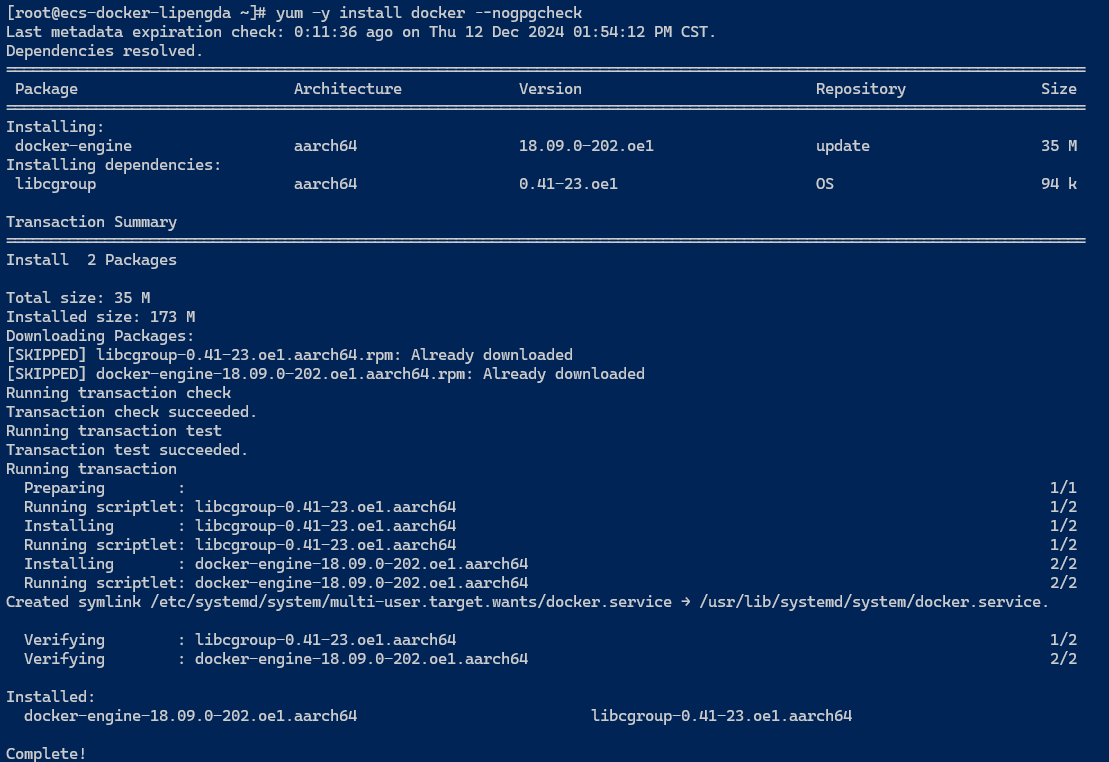
\includegraphics[width=0.9\textwidth]{img/1.5.1.png}
\caption{安装Docker}
\end{figure}

启动Docker 后台服务。

\begin{lstlisting}[language=bash]
    systemctl start docker
\end{lstlisting}

\subsubsection{配置镜像加速}

在华为云 所有服务 \(\to\) 容器 \(\to\) 容器镜像服务SWR \(\to\) 镜像资源 \(\to\) 镜像中心 \(\to\) 镜像加速器,复制加速器地址。

\begin{figure}[H]
\centering
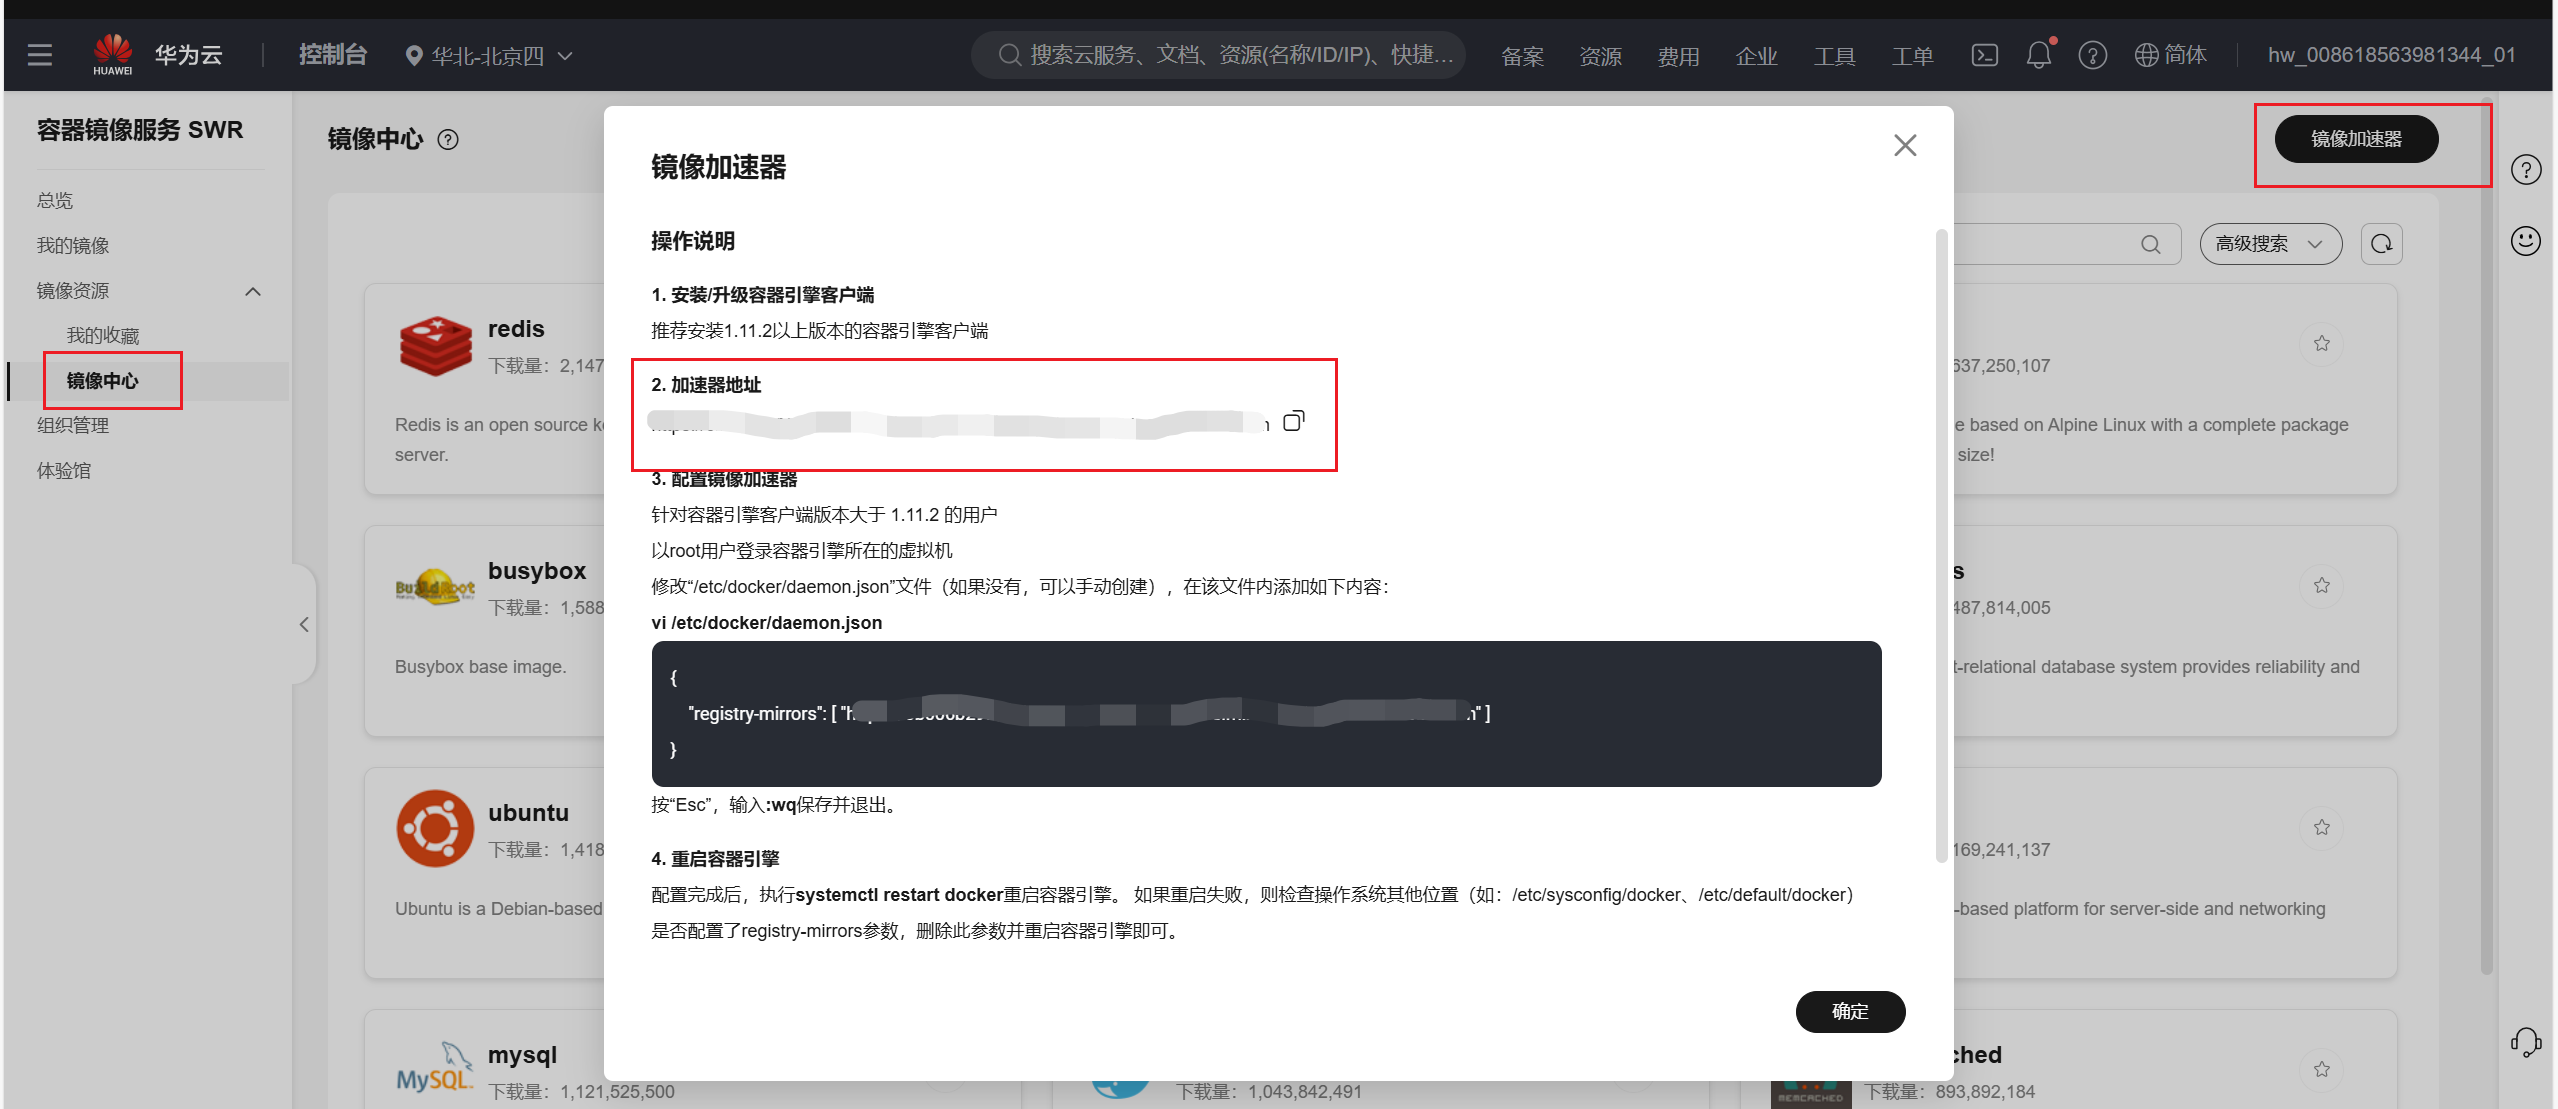
\includegraphics[width=0.9\textwidth]{img/1.6.1.png}
\caption{复制镜像加速器地址}
\end{figure}

修改 Docker 配置文件。

\begin{lstlisting}[language=bash]
    vi /etc/docker/daemon.json
\end{lstlisting}

添加如下内容:

\begin{lstlisting}[language=bash]
    {
        "registry-mirrors": ["加速器地址"]
    }
\end{lstlisting}

保存退出后,重启 Docker 服务。

\begin{lstlisting}[language=bash]
    systemctl daemon-reload
    systemctl restart docker
\end{lstlisting}

\subsubsection{测试Docker}

测试运行 hello-world 镜像。

\begin{lstlisting}[language=bash]
    docker run hello-world
\end{lstlisting}

\begin{figure}[H]
\centering
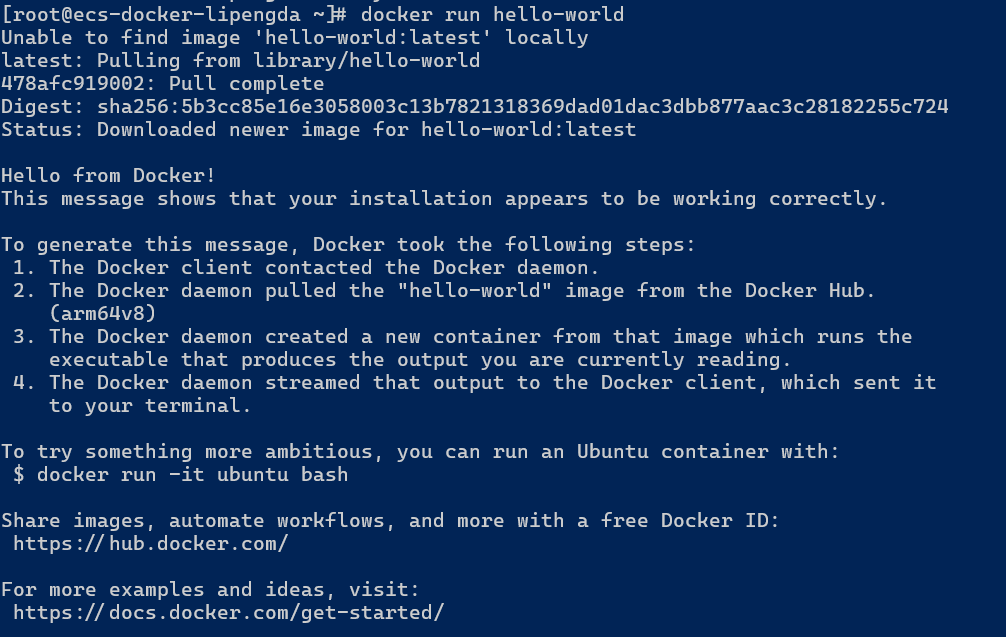
\includegraphics[width=0.9\textwidth]{img/1.7.1.png}
\caption{运行hello-world镜像}
\end{figure}

查看下载的hello-world镜像。

\begin{lstlisting}[language=bash]
    docker images
\end{lstlisting}

\begin{figure}[H]
\centering
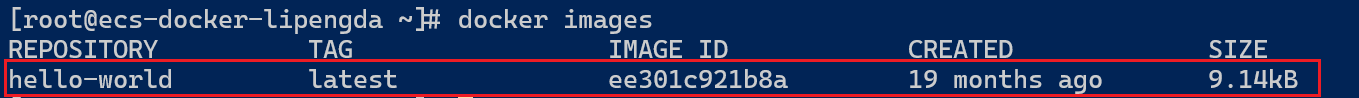
\includegraphics[width=0.9\textwidth]{img/0.3.png}
\caption{查看下载的hello-world镜像}
\end{figure}

\subsection{镜像的基本操作}

\label{subsec:image-management}

\subsubsection{获取镜像}

下载 nginx 镜像

\begin{lstlisting}[language=bash]
    docker pull nginx
\end{lstlisting}

\begin{figure}[H]
\centering
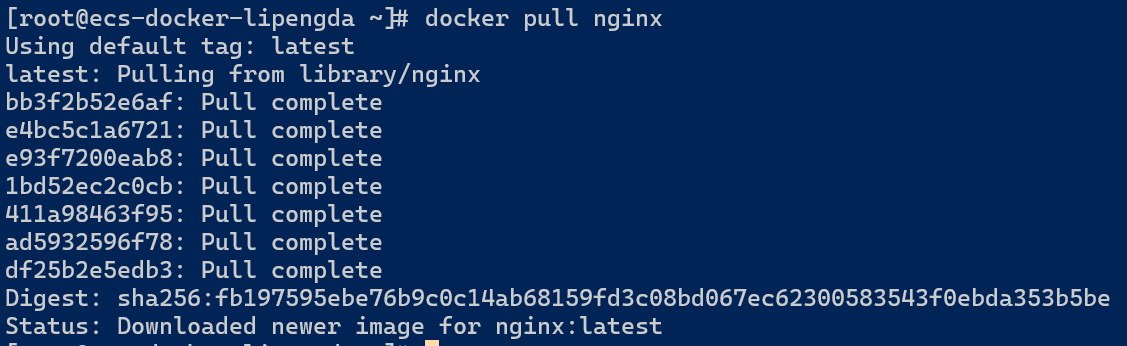
\includegraphics[width=0.9\textwidth]{img/2.3.1.1.png}
\caption{下载nginx镜像}
\end{figure}

\subsubsection{查询及删除镜像}

查询已经下载的镜像

\begin{lstlisting}[language=bash]
    docker images
\end{lstlisting}

或

\begin{lstlisting}[language=bash]
    docker image ls
\end{lstlisting}

\begin{figure}[H]
\centering
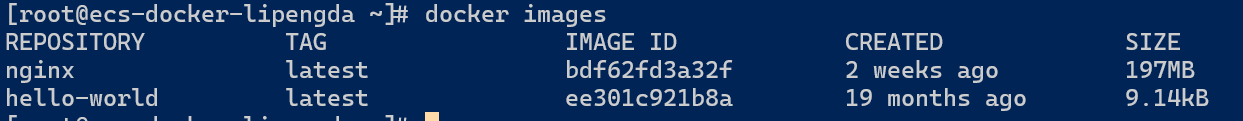
\includegraphics[width=0.9\textwidth]{img/0.2.3.2.1.png}
\caption{查询已下载的镜像}
\end{figure}

查询部分镜像

\begin{lstlisting}[language=bash]
    docker image ls nginx
\end{lstlisting}

\begin{figure}[H]
\centering
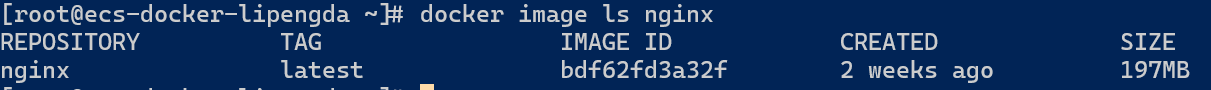
\includegraphics[width=0.9\textwidth]{img/0.2.3.2.2.png}
\caption{查询部分镜像}
\end{figure}

查看镜像的大小

\begin{lstlisting}[language=bash]
    docker system df
\end{lstlisting}

\begin{figure}[H]
\centering
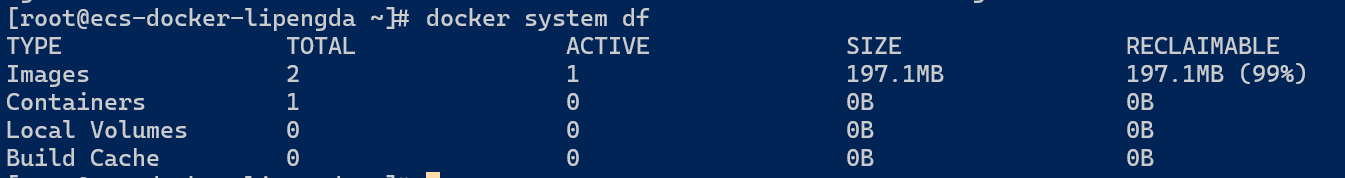
\includegraphics[width=0.9\textwidth]{img/0.2.3.2.3.png}
\caption{查看镜像的大小}
\end{figure}

通过短ID或完整ID删除镜像

\begin{lstlisting}[language=bash]
    docker images
    docker rmi <ID>
\end{lstlisting}

\begin{figure}[H]
\centering
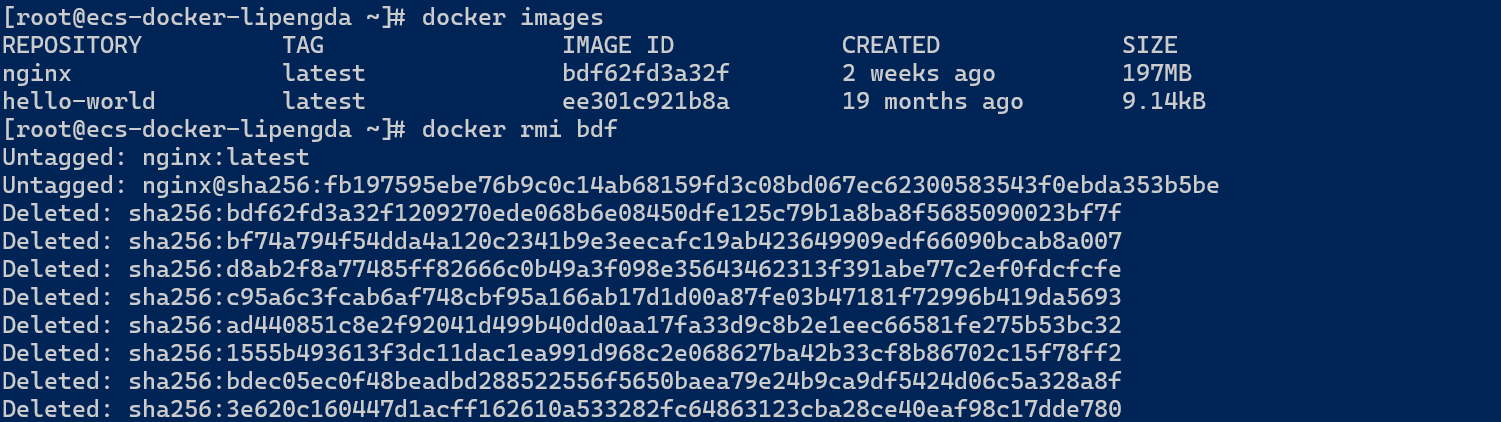
\includegraphics[width=0.9\textwidth]{img/0.2.3.2.4.png}
\caption{删除镜像}
\end{figure}

通过仓库名+标签删除镜像,如果删除的镜像已经产生了容器实例,不管容器实例是否启动都会提示无法删除,因为镜像被占用。这时需要先删除容器实例或添加删除参数 \texttt{-f} 强制删除。

\begin{figure}[H]
\centering
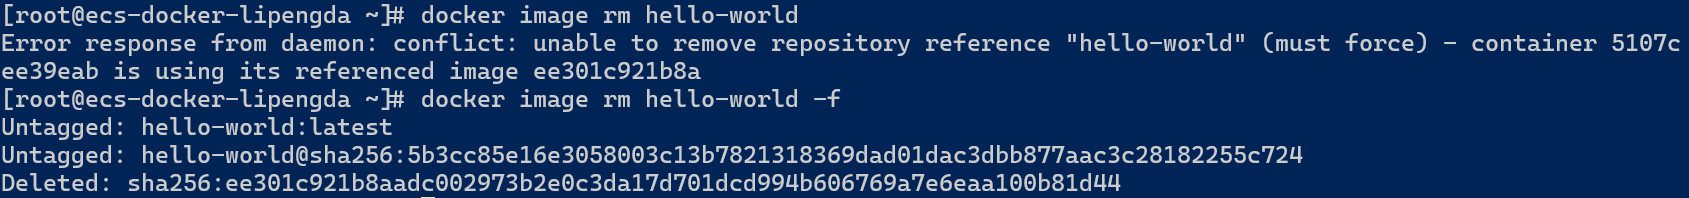
\includegraphics[width=0.9\textwidth]{img/0.2.3.2.5.png}
\caption{删除镜像}
\end{figure}

\subsection{容器的基本操作}
\label{subsec:container-management}

\subsubsection{容器的创建与启停}

创建一个基于httpd镜像的新容器。若主机中没有对应镜像,将会从docker Hub中拉取最新镜像。

\begin{lstlisting}[language=bash]
    docker create httpd
\end{lstlisting}

\begin{figure}[H]
\centering
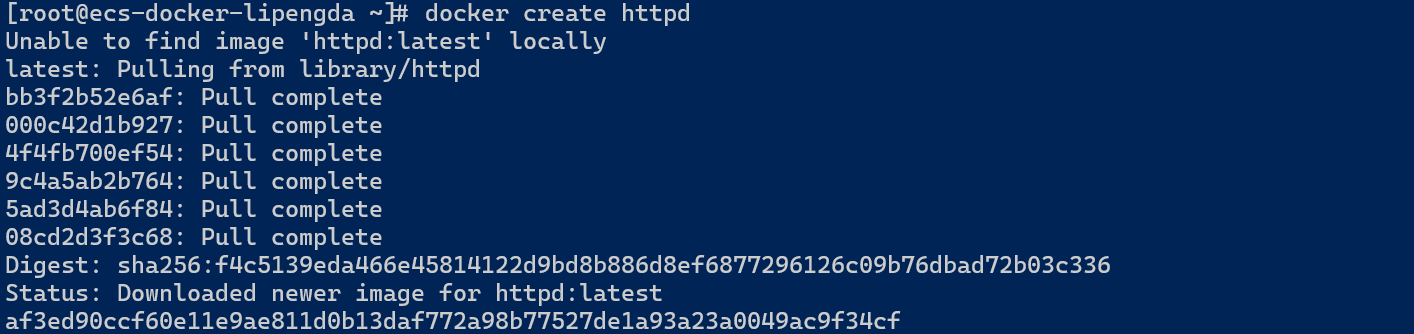
\includegraphics[width=0.9\textwidth]{img/0.2.4.1.1.png}
\caption{创建容器}
\end{figure}

查看容器信息

\begin{lstlisting}[language=bash]
    docker ps -a
\end{lstlisting}

\begin{figure}[H]
\centering
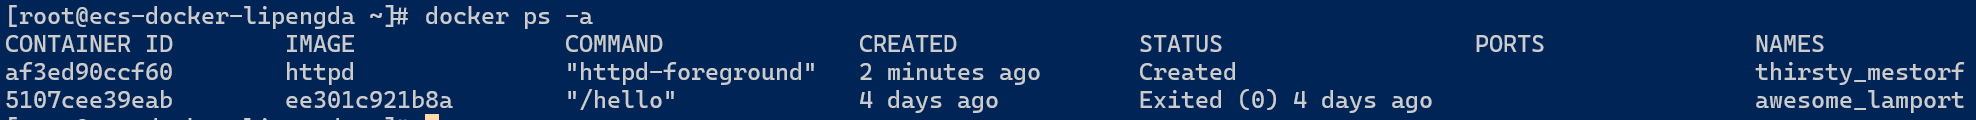
\includegraphics[width=0.9\textwidth]{img/0.2.4.1.2.png}
\caption{查看容器信息}
\end{figure}

可以看到容器 ID 为 \texttt{af3ed90ccf60},名称为 \texttt{thirsty\_mestorf}

根据显示的容器ID或容器名称启动容器

\begin{lstlisting}[language=bash]
    docker start af3ed90ccf60
    docker ps -a
\end{lstlisting}

\begin{figure}[H]
\centering
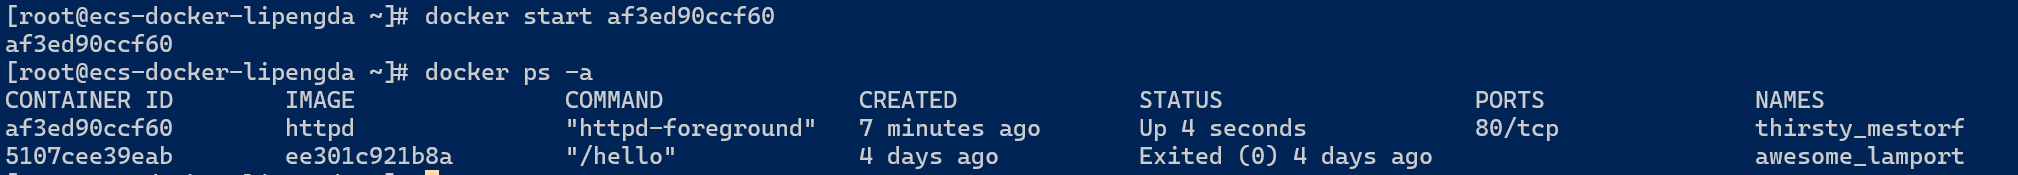
\includegraphics[width=0.9\textwidth]{img/0.2.4.1.3.png}
\caption{启动容器}
\end{figure}

停止容器运行

\begin{lstlisting}[language=bash]
    docker stop af3ed90ccf60
    docker ps -a
\end{lstlisting}

\begin{figure}[H]
\centering
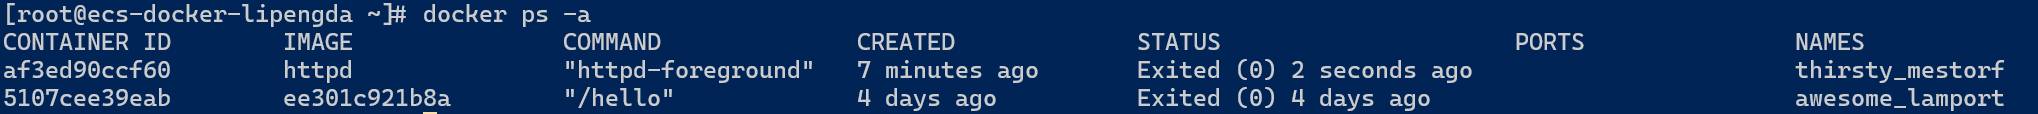
\includegraphics[width=0.9\textwidth]{img/0.2.4.1.4.png}
\caption{停止容器}
\end{figure}

重启容器

\begin{lstlisting}[language=bash]
    docker restart af3ed90ccf60
    docker ps -a
\end{lstlisting}

\begin{figure}[H]
\centering
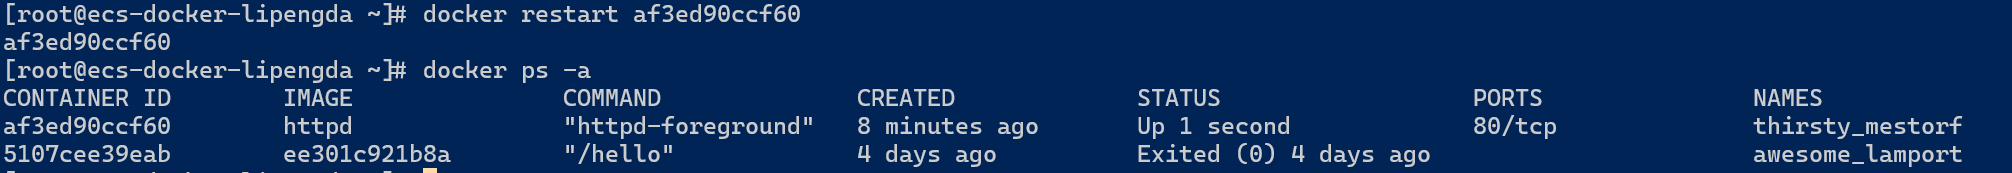
\includegraphics[width=0.9\textwidth]{img/0.2.4.1.5.png}
\caption{重启容器}
\end{figure}

暂停容器

\begin{lstlisting}[language=bash]
    docker pause af3ed90ccf60
    docker ps -a
\end{lstlisting}

\begin{figure}[H]
\centering
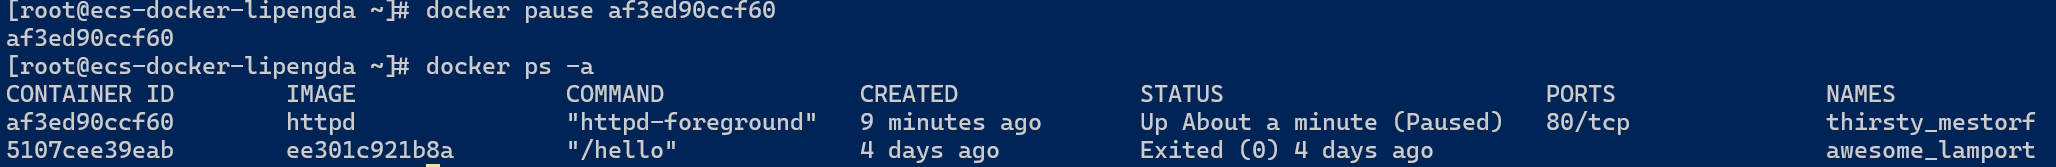
\includegraphics[width=0.9\textwidth]{img/0.2.4.1.6.png}
\caption{暂停容器}
\end{figure}

恢复暂停的容器

\begin{lstlisting}[language=bash]
    docker unpause af3ed90ccf60
    docker ps -a
\end{lstlisting}

\begin{figure}[H]
\centering
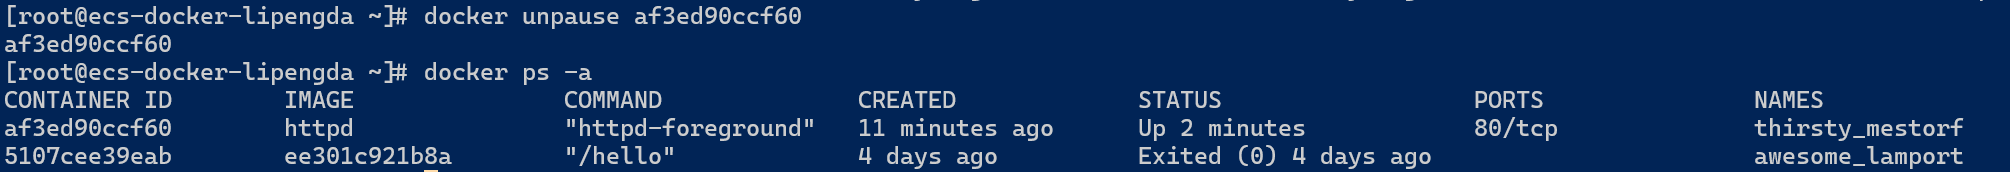
\includegraphics[width=0.9\textwidth]{img/0.2.4.1.7.png}
\caption{恢复暂停的容器}
\end{figure}

强制停止容器

\begin{lstlisting}[language=bash]
    docker kill af3ed90ccf60
    docker ps -a
\end{lstlisting}

\begin{figure}[H]
\centering
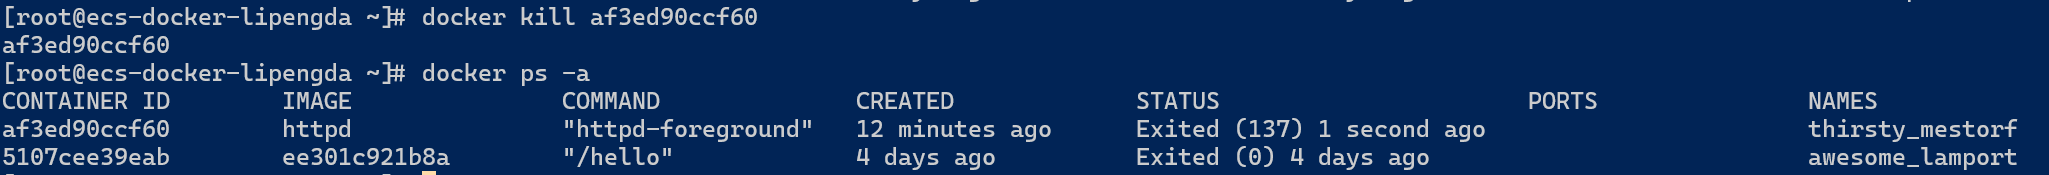
\includegraphics[width=0.9\textwidth]{img/0.2.4.1.8.png}
\caption{强制停止容器}
\end{figure}

启动容器,给容器重新命名

\begin{lstlisting}[language=bash]
    docker start af3ed90ccf60
    docker ps -a
    docker rename af3ed90ccf60 myhttpd
    docker ps -a
\end{lstlisting}

\begin{figure}[H]
\centering
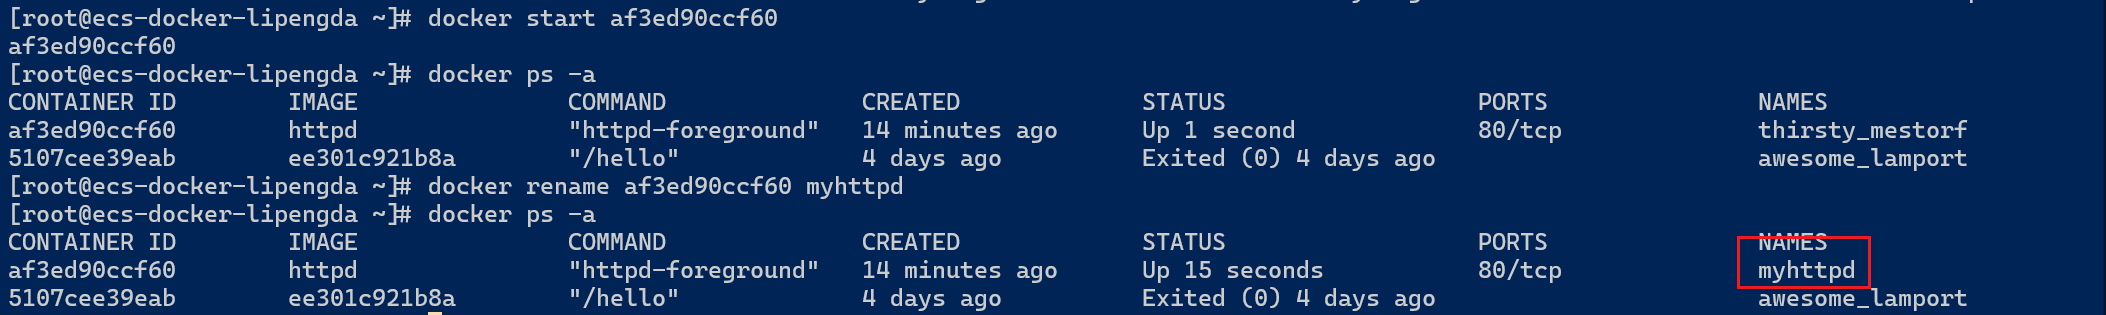
\includegraphics[width=0.9\textwidth]{img/0.2.4.1.9.png}
\caption{给容器重新命名}
\end{figure}

\subsubsection{容器的运行}

运行一个新容器,该容器基于ubuntu:14.04。

\begin{lstlisting}[language=bash]
    docker run ubuntu:14.04 /bin/echo 'Hello world'
\end{lstlisting}

\begin{figure}[H]
\centering
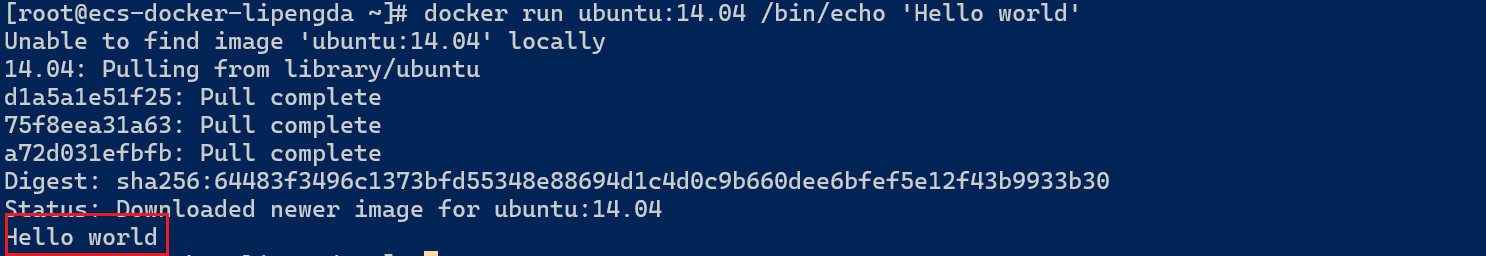
\includegraphics[width=0.9\textwidth]{img/0.2.4.2.1.png}
\caption{运行容器}
\end{figure}

下面的命令则启动一个 bash 终端,允许用户进行交互。

\begin{lstlisting}[language=bash]
    docker run -it ubuntu:14.04 /bin/bash
\end{lstlisting}

执行一些命令

\begin{lstlisting}[language=bash]
    pwd
    ls
\end{lstlisting}

退出容器

\begin{lstlisting}[language=bash]
    exit
\end{lstlisting}

\begin{figure}[H]
\centering
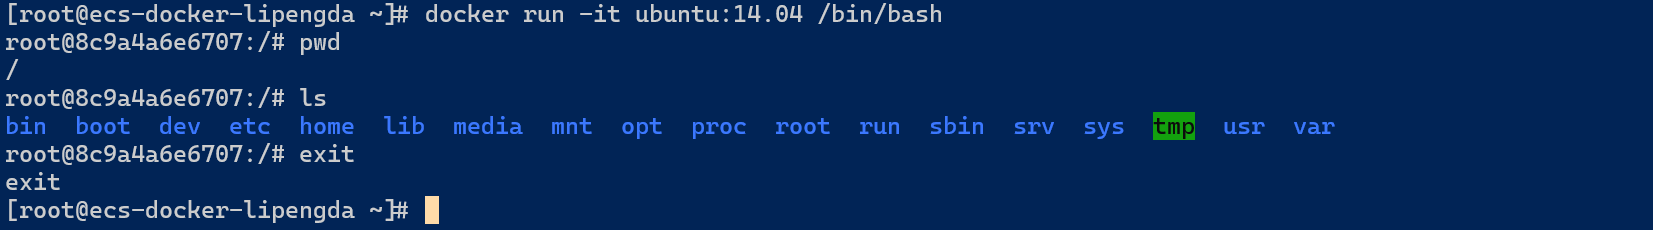
\includegraphics[width=0.9\textwidth]{img/0.2.4.2.2.png}
\caption{运行容器启动一个 bash 终端}
\end{figure}

使用 \texttt{-d} 参数,在后台运行容器

\begin{lstlisting}[language=bash]
    docker run ubuntu:14.04 /bin/sh -c "while true; do echo hello world; sleep 1; done"
    docker run -d ubuntu:14.04 /bin/sh -c "while true; do echo hello world; sleep 1; done"
\end{lstlisting}

\begin{figure}[H]
\centering
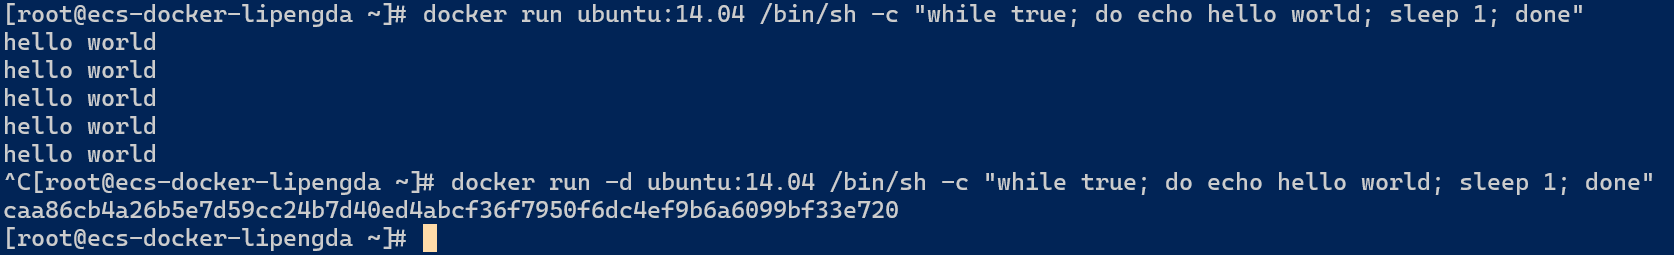
\includegraphics[width=0.9\textwidth]{img/0.2.4.2.3.png}
\caption{在后台运行容器}
\end{figure}

获取容器的日志

\begin{lstlisting}[language=bash]
    docker logs caa86cb4a26b
\end{lstlisting}

\begin{figure}[H]
\centering
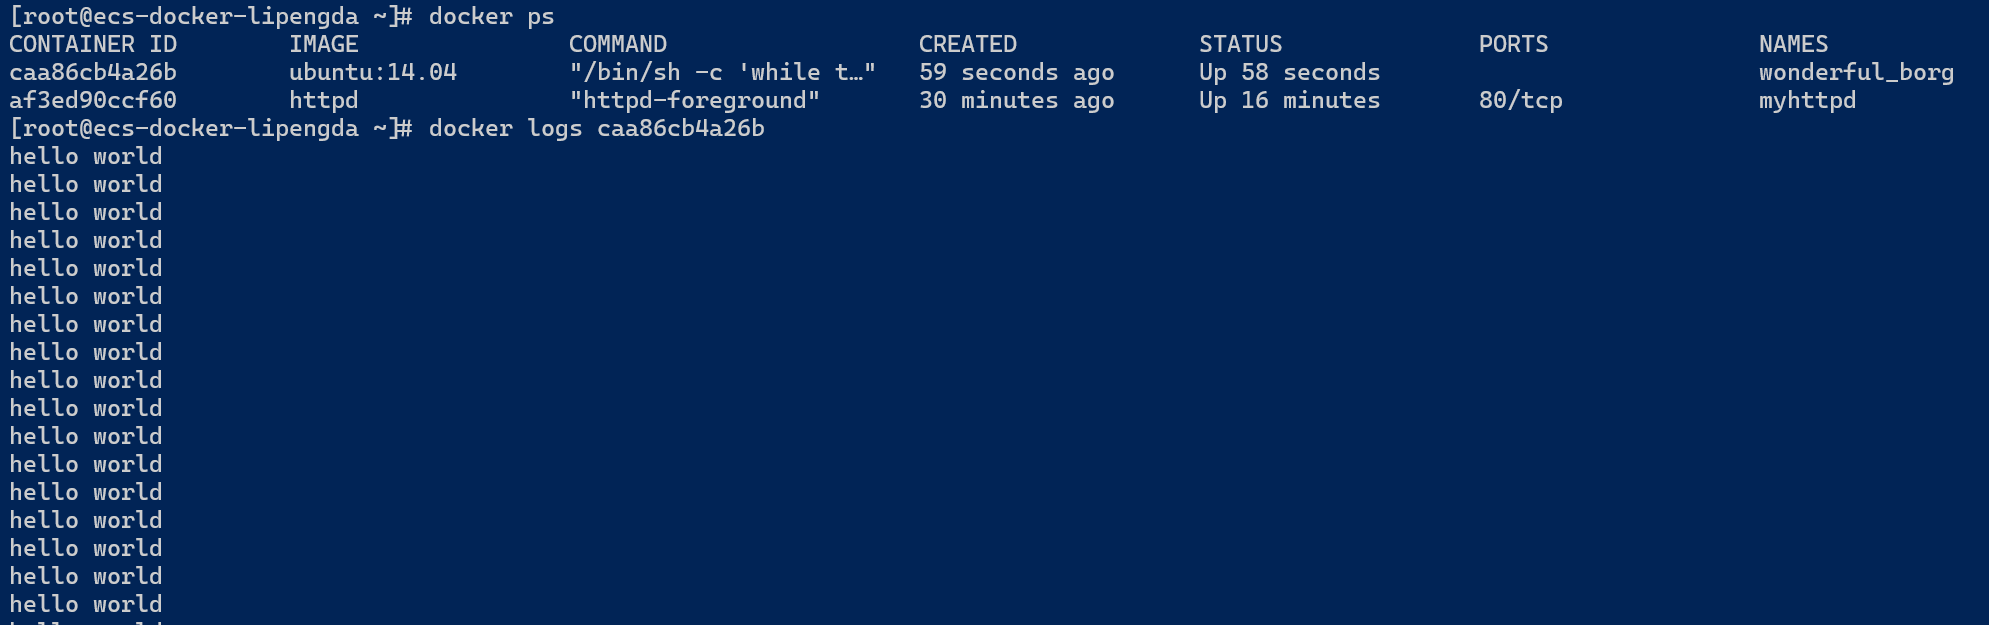
\includegraphics[width=0.9\textwidth]{img/0.2.4.2.4.png}
\caption{获取容器的日志}
\end{figure}

\subsubsection{进入容器}

某些时候需要进入容器进行操作,可以使用docker attach命令或docker exec命令。

启动一个容器

\begin{lstlisting}[language=bash]
    docker run -dit ubuntu:14.04
    docker ps 
\end{lstlisting}

\begin{figure}[H]
\centering
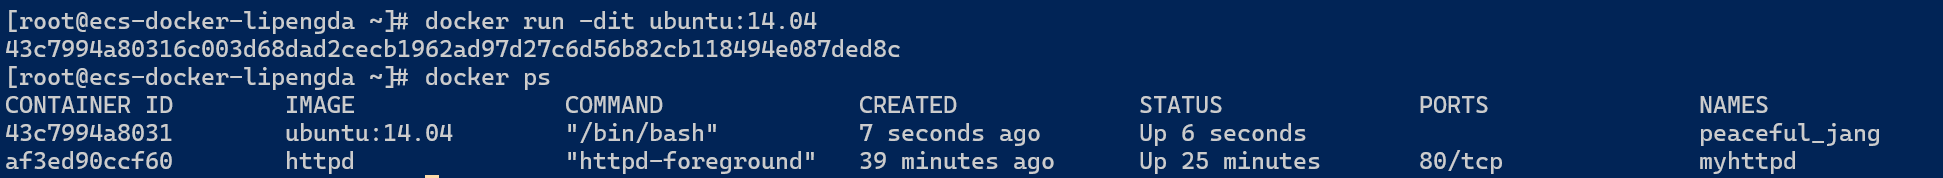
\includegraphics[width=0.9\textwidth]{img/0.2.4.3.1.png}
\caption{启动一个容器}
\end{figure}

使用attach命令,直接进入容器启动命令的终端。

\begin{lstlisting}[language=bash]
    docker attach 43c7994a8031
\end{lstlisting}

执行一些命令

\begin{lstlisting}[language=bash]
    ps
    exit
\end{lstlisting}

\begin{figure}[H]
\centering
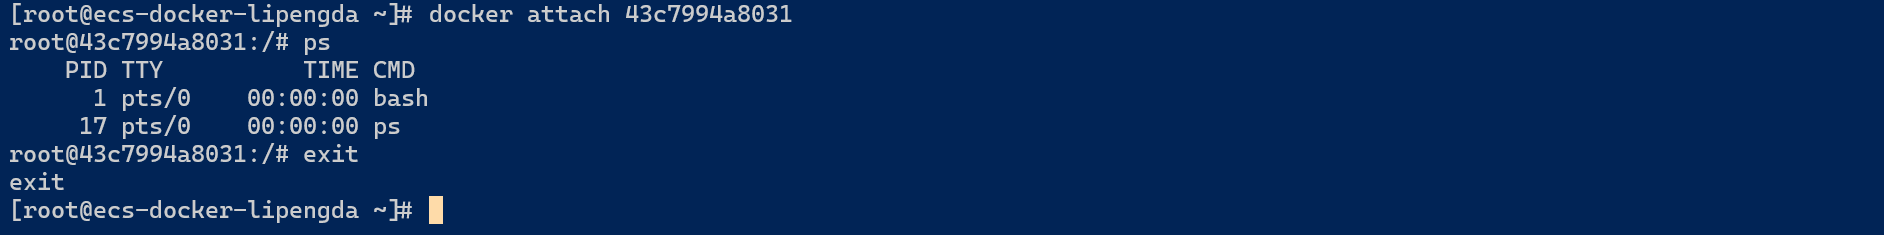
\includegraphics[width=0.9\textwidth]{img/0.2.4.3.2.png}
\caption{使用attach命令进入容器}
\end{figure}

启动一个新容器

\begin{lstlisting}[language=bash]
    docker run -dit ubuntu:14.04
    docker ps
\end{lstlisting}

\begin{figure}[H]
\centering
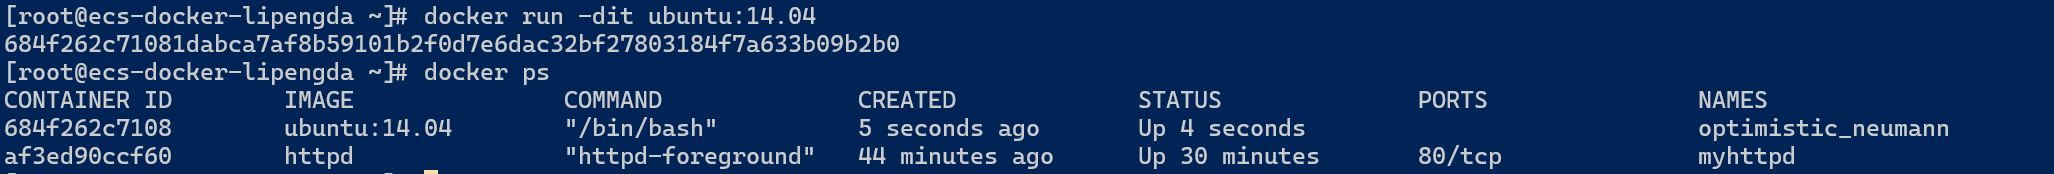
\includegraphics[width=0.9\textwidth]{img/0.2.4.3.3.png}
\caption{启动一个新容器}
\end{figure}

通过docker exec进入容器

\begin{lstlisting}[language=bash]
    docker exec -it 684f262c7108 bash
\end{lstlisting}

执行一些命令

\begin{lstlisting}[language=bash]
    ps
    exit
\end{lstlisting}

\begin{figure}[H]
\centering
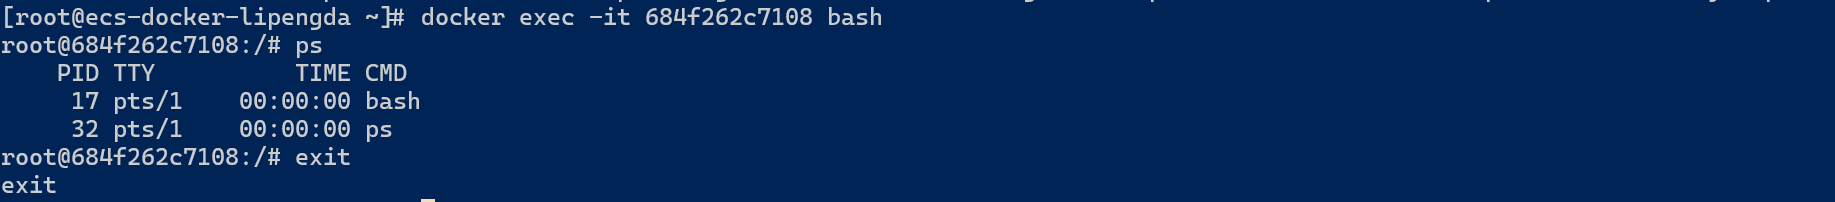
\includegraphics[width=0.9\textwidth]{img/0.2.4.3.4.png}
\caption{通过docker exec进入容器}
\end{figure}

\subsubsection{删除容器}

使用docker rm 来删除一个处于终止状态的容器。若容器没有退出则无法删除,需要先停止容器。

\begin{lstlisting}[language=bash]
    docker ps
    docker rm <ID>
    docker stop <ID>
    docker rm <ID>
    docker ps
\end{lstlisting}

\begin{figure}[H]
\centering
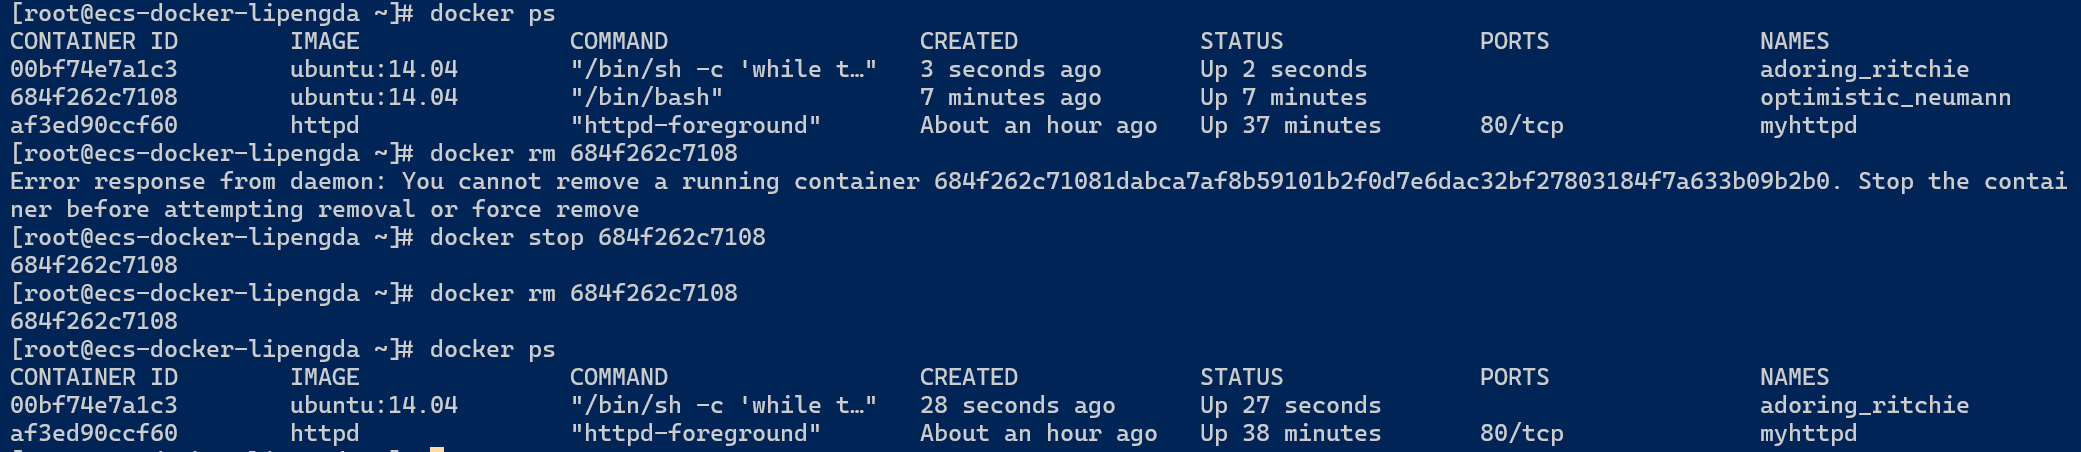
\includegraphics[width=0.9\textwidth]{img/0.2.4.4.1.png}
\caption{删除容器}
\end{figure}

使用docker rm -f来删除一个处于运行状态的容器。

\begin{lstlisting}[language=bash]
    docker ps
    docker rm -f <ID>
    docker ps
\end{lstlisting}

\begin{figure}[H]
\centering
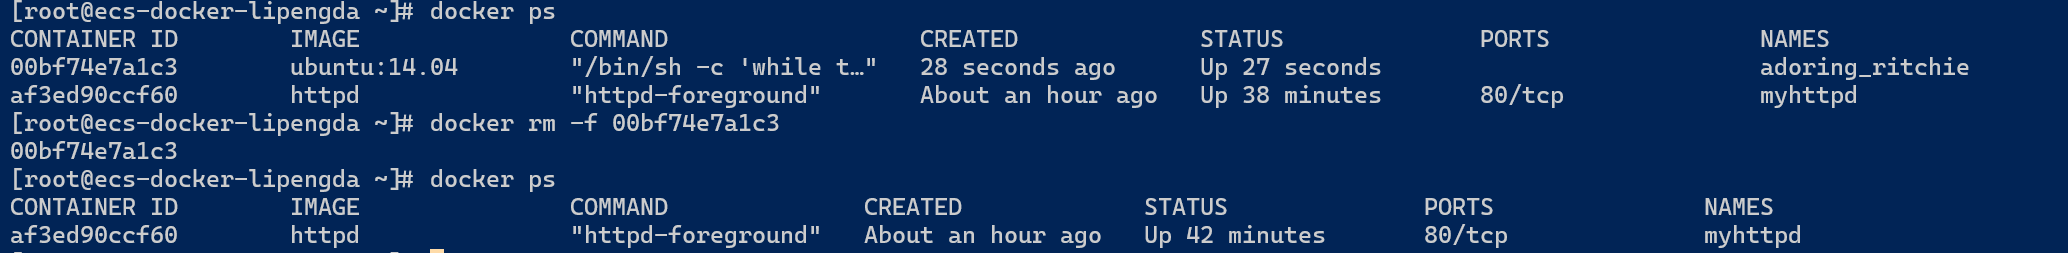
\includegraphics[width=0.9\textwidth]{img/0.2.4.4.2.png}
\caption{删除容器}
\end{figure}

删除所有已终止的容器。

\begin{lstlisting}[language=bash]
    docker rm -v $(docker ps -aq -f status=exited)
\end{lstlisting}

\begin{figure}[H]
\centering
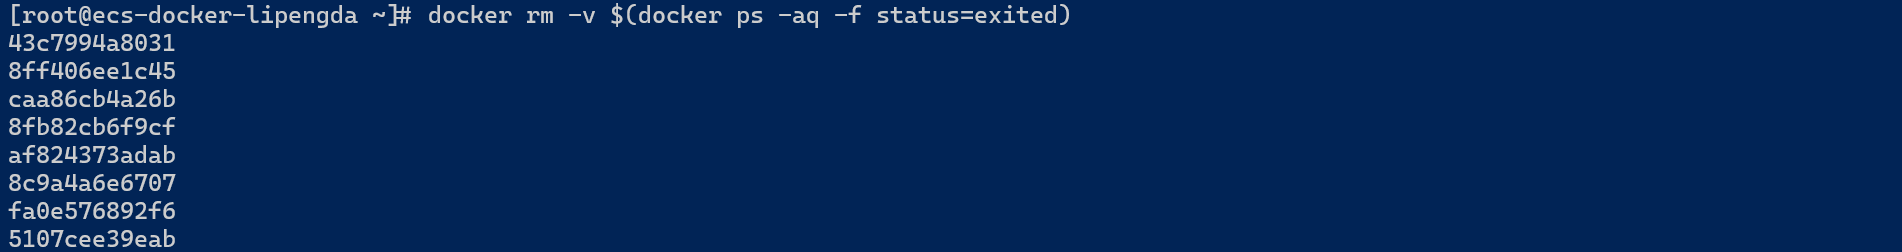
\includegraphics[width=0.9\textwidth]{img/0.2.4.4.3.png}
\caption{删除所有已终止的容器}
\end{figure}

\subsection{私有镜像仓库搭建}

\subsubsection{安装运行docker-registry}

获取官方registry 镜像并运行容器。

\begin{lstlisting}[language=bash]
    docker run -d -p 5000:5000 --restart=always --name registry registry
\end{lstlisting}

\begin{figure}[H]
\centering
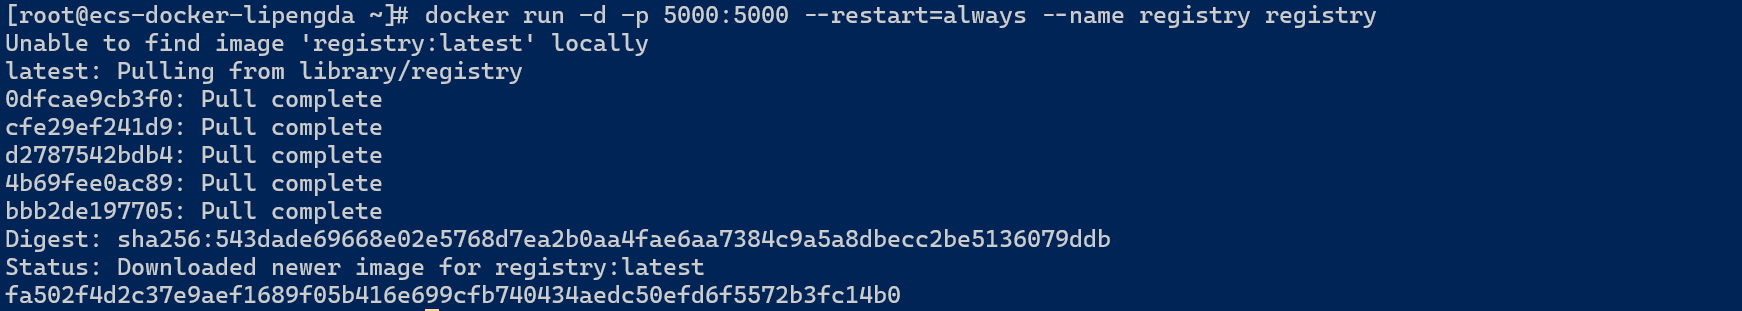
\includegraphics[width=0.9\textwidth]{img/2.5.1.1.png}
\caption{获取官方registry 镜像并运行容器}
\end{figure}

在本机查看已有的镜像。

\begin{lstlisting}[language=bash]
    docker images
\end{lstlisting}

\begin{figure}[H]
\centering
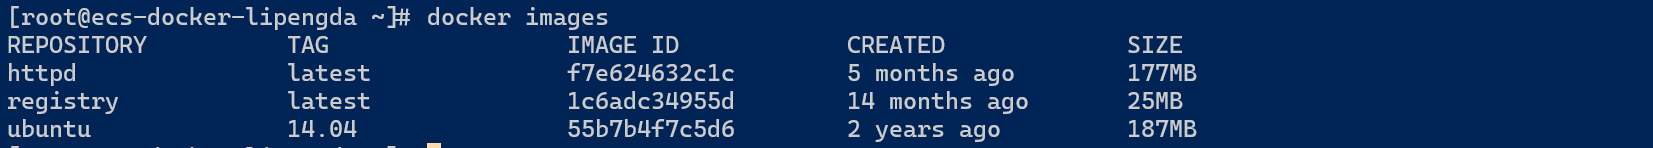
\includegraphics[width=0.9\textwidth]{img/2.5.1.2.png}
\caption{查看已有的镜像}
\end{figure}

通过docker tag命令将基础镜像ubuntu:14.04镜像进行标记。

\begin{lstlisting}[language=bash]
    docker tag ubuntu:14.04 127.0.0.1:5000/myubuntu:14.04
    docker images
\end{lstlisting} 

\begin{figure}[H]
\centering
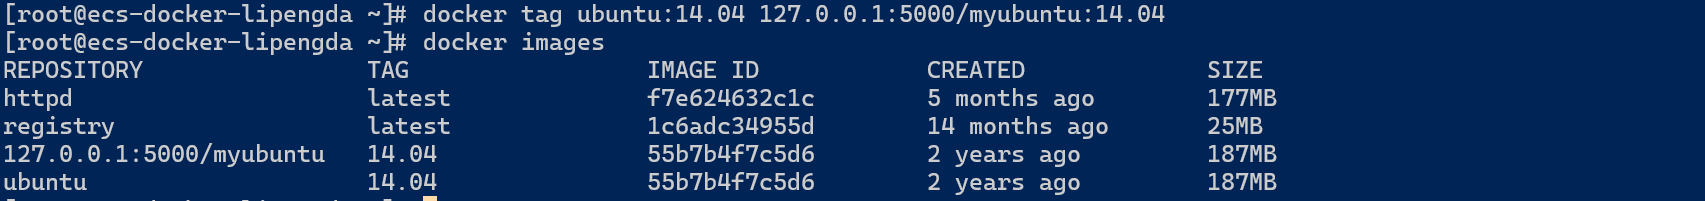
\includegraphics[width=0.9\textwidth]{img/2.5.1.3.png}
\caption{标记镜像}
\end{figure}

使用docker push 上传标记的镜像。

\begin{lstlisting}[language=bash]
    docker push 127.0.0.1:5000/myubuntu:14.04
\end{lstlisting}

\begin{figure}[H]
\centering
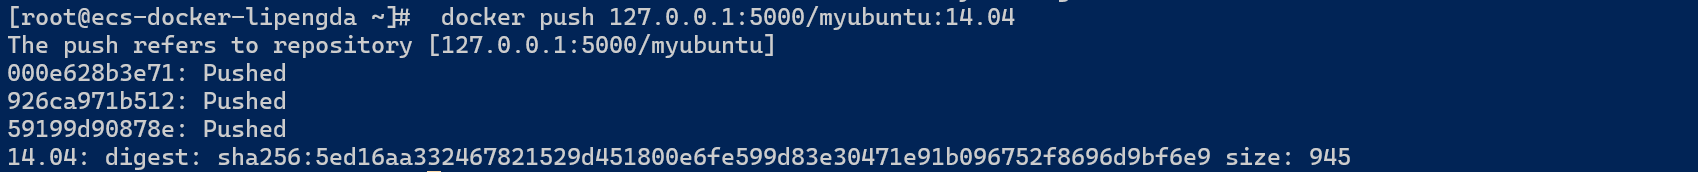
\includegraphics[width=0.9\textwidth]{img/2.5.1.4.png}
\caption{上传镜像}
\end{figure}

用curl查看仓库中的镜像。

\begin{lstlisting}[language=bash]
    curl 127.0.0.1:5000/v2/_catalog
\end{lstlisting}

\begin{figure}[H]
\centering
\includegraphics[width=0.9\textwidth]{img/0.2.5.1.5.png}
\caption{查看仓库中的镜像}
\end{figure}

删除已有镜像,再尝试从私有仓库中下载这个镜像

\begin{lstlisting}[language=bash]
    docker image rm 127.0.0.1:5000/myubuntu:14.04
    docker images
    docker pull 127.0.0.1:5000/myubuntu:14.04
    docker images
\end{lstlisting}

\begin{figure}[H]
\centering
\includegraphics[width=0.9\textwidth]{img/2.5.1.6.png}
\caption{重新下载镜像}
\end{figure}

\subsection{Dockerfile 文件构建}

\subsubsection{构建 nginx}

下载基础镜像centos:7

\begin{lstlisting}[language=bash]
    docker pull centos:7
\end{lstlisting}

创建nginx\_demo文件夹

\begin{lstlisting}[language=bash]
    pwd
    mkdir nginx_demo
    ls
\end{lstlisting}

\begin{figure}[H]
\centering
\includegraphics[width=0.9\textwidth]{img/0.2.5.1.5.png}
\caption{创建nginx\_demo文件夹}
\end{figure}

进入文件夹,下载nginx源码压缩包。

\begin{lstlisting}[language=bash]
    cd nginx_demo
    wget http://nginx.org/download/nginx-1.12.2.tar.gz
\end{lstlisting}

\begin{figure}[H]
\centering
\includegraphics[width=0.9\textwidth]{img/2.7.1.2.png}
\caption{下载nginx源码压缩包}
\end{figure}

创建 Dockerfile 文件。

\begin{lstlisting}[language=bash]
    vim Dockerfile
\end{lstlisting}

输入以下内容。

由于 centos 7 已经停止维护,其中的 yum 源已经失效,需要修改 yum 源。

\begin{lstlisting}[language=bash]
    # base image
    FROM centos:7
    
    # MAINTAINER
    MAINTAINER lipengda
    
    # put nginx-1.12.2.tar.gz into /usr/local/src and unpack nginx
    ADD nginx-1.12.2.tar.gz /usr/local/src

^+  RUN sed -i s/^#.*baseurl=http/baseurl=http/g /etc/yum.repos.d/*.repo
^+  RUN sed -i s/^mirrorlist=http/#mirrorlist=http/g /etc/yum.repos.d/*.repo
^+  RUN sed -i s/mirror.centos.org/vault.centos.org/g /etc/yum.repos.d/*.repo

    # running required command
    RUN yum install -y gcc gcc-c++ glibc make autoconf openssl openssl-devel 
    RUN yum install -y libxslt-devel -y gd gd-devel GeoIP GeoIP-devel pcre pcre-devel
    RUN useradd -M -s /sbin/nologin nginx
    
    # change dir to /usr/local/src/nginx-1.12.2
    WORKDIR /usr/local/src/nginx-1.12.2
    
    # execute command to compile nginx
    RUN ./configure \
    --user=nginx --group=nginx \
    --prefix=/usr/local/nginx --with-file-aio \
    --with-http_ssl_module \
    --with-http_realip_module \
    --with-http_addition_module \
    --with-http_xslt_module \
    --with-http_image_filter_module \
    --with-http_geoip_module \
    --with-http_sub_module  \
    --with-http_dav_module \
    --with-http_flv_module \
    --with-http_mp4_module \
    --with-http_gunzip_module \ 
    --with-http_gzip_static_module \
    --with-http_auth_request_module \
    --with-http_random_index_module  \
    --with-http_secure_link_module \
    --with-http_degradation_module  \
    --with-http_stub_status_module && make && make install
    
    RUN chmod -R 755 /usr/local/nginx/
    
    EXPOSE 80
\end{lstlisting}

通过Dockerfile创建nginx镜像。

\begin{lstlisting}[language=bash]
    docker build -t my_nginx:v1 .
\end{lstlisting}

\begin{figure}[H]
\centering
\includegraphics[width=0.9\textwidth]{img/2.7.1.3.1.png}
\caption{创建nginx镜像(1)}
\end{figure}

\begin{figure}[H]
\centering
\includegraphics[width=0.9\textwidth]{img/2.7.1.3.2.png}
\caption{创建nginx镜像(2)}
\end{figure}

查看构建的镜像。

\begin{lstlisting}[language=bash]
    docker images
\end{lstlisting}

\begin{figure}[H]
\centering
\includegraphics[width=0.9\textwidth]{img/2.7.1.4.png}
\caption{查看构建的镜像}
\end{figure}

\subsubsection{nginx镜像验证}

通过构建的镜像,运行一个容器,将端口进行映射。

\begin{lstlisting}[language=bash]
    docker run -d -p 80:80 my_nginx:v1 /usr/local/nginx/sbin/nginx -g "daemon off;"
\end{lstlisting}

查看容器状态

\begin{lstlisting}[language=bash]
    docker ps
\end{lstlisting}

\begin{figure}[H]
\centering
\includegraphics[width=0.9\textwidth]{img/2.7.2.1.png}
\caption{运行容器并查看容器状态}
\end{figure}

打开浏览器,输入ecs-docker弹性IP地址,默认端口为80,进行验证,显示“Welcome to nginx!”,说明容器运行正常。

\begin{figure}[H]
\centering
\includegraphics[width=0.9\textwidth]{img/0.2.7.2.2.png}
\caption{验证nginx镜像}
\end{figure}

\subsubsection{Dockerfile指令的添加}

我们也可以基于以上Dockerfile文件依次添加其他的指令进行构建,比如我们可以添加CMD命令,设置nginx非daemon守护进程,这样容器启动时不会自动退出。

\begin{lstlisting}[language=bash]
    vim Dockerfile
\end{lstlisting}

在原有Dockerfile基础上,增加如下内容到Dockerfile最后一行。

\begin{lstlisting}[language=bash]
    CMD /usr/local/nginx/sbin/nginx -g "daemon off;"
\end{lstlisting}

重新构建镜像。

\begin{lstlisting}[language=bash]
    docker build -t my_nginx:v2 .
\end{lstlisting}

\begin{figure}[H]
\centering
\includegraphics[width=0.9\textwidth]{img/2.7.3.1.png}
\caption{重新构建镜像}
\end{figure}

查看构建的镜像。 

\begin{lstlisting}[language=bash]
    docker images
\end{lstlisting}

\begin{figure}[H]
\centering
\includegraphics[width=0.9\textwidth]{img/2.7.3.2.png}
\caption{查看构建的镜像}
\end{figure}

通过构建的镜像,运行一个容器,将端口进行映射,将容器的80端口映射到主机的81端口。

\begin{lstlisting}[language=bash]
    docker run -d -p 81:80 my_nginx:v2
\end{lstlisting}

查看容器状态

\begin{lstlisting}[language=bash]
    docker ps
\end{lstlisting}

\begin{figure}[H]
\centering
\includegraphics[width=0.9\textwidth]{img/2.7.3.3.png}
\caption{运行容器并查看容器状态}
\end{figure}

打开浏览器进行验证,打开浏览器,输入弹性IP地址,端口为81,进行验证,显示“Welcome to nginx!”,说明容器运行正常。

\begin{figure}[H]
\centering
\includegraphics[width=0.9\textwidth]{img/0.2.7.3.4.png}
\caption{验证nginx镜像}
\end{figure}

\subsection{删除弹性云服务器及相关资源}

打开云服务器控制台,在需要删除的云服务器后面选择“更多>删除”。步骤 2	在弹出对话框中勾选“释放云服务器绑定的弹性公网IP地址”和“删除云服务器挂载的数据盘”,然后点击“是”。

\begin{figure}[H]
\centering
\includegraphics[width=0.9\textwidth]{img/2.8.1.1.png}
\caption{删除云服务器}
\end{figure}

查看到列表中已没有资源时,表示弹性云服务器已删除。

\begin{figure}[H]
\centering
\includegraphics[width=0.9\textwidth]{img/2.8.1.2.png}
\caption{删除完成}
\end{figure}

\section{实验结果}


本次实验中,我们成功完成了鲲鹏云容器的安装和配置,并掌握了 Docker 的基本操作。以下是实验过程中取得的主要结果。

\subsection{创建云服务器}

在鲲鹏云容器控制台中,成功创建了一个云服务器,如图 \ref{fig:create-server} 所示。

\begin{figure}[H]
\centering
\includegraphics[width=0.9\textwidth]{img/0.1.png}
\caption{创建云服务器}
\label{fig:create-server}
\end{figure}

\subsection{登录云服务器}

成功登录到云服务器,验证了服务器的正常运行情况,如图 \ref{fig:login-server} 所示。

\begin{figure}[H]
\centering
\includegraphics[width=0.9\textwidth]{img/0.2.png}
\caption{登录云服务器}
\label{fig:login-server}
\end{figure}

\subsection{查看已下载的镜像}

使用命令 \texttt{docker images} 查看已经下载的镜像,可以看到 \texttt{hello-world} 镜像已经成功下载,如图 \ref{fig:docker-images} 所示。

\begin{figure}[H]
\centering
\includegraphics[width=0.9\textwidth]{img/0.3.png}
\caption{查看已下载的镜像}
\label{fig:docker-images}
\end{figure}

\subsection{镜像的基本操作}

通过执行镜像的查询、下载和删除等操作,加深了对镜像管理的理解。详细的操作过程和结果可参考第 \ref{subsec:image-management}(点击以跳转) 节。

\subsection{容器的基本操作}

掌握了容器的创建、启动、停止、删除等基本操作。具体的步骤和结果请参见第 \ref{subsec:container-management} 节。

\subsection{查看私有仓库中的镜像}

在搭建私有镜像仓库后,使用 \texttt{curl} 命令查看仓库中的镜像,成功获取到了仓库中包含的镜像列表,如图 \ref{fig:registry-images} 所示。

\begin{figure}[H]
\centering
\includegraphics[width=0.9\textwidth]{img/0.2.5.1.5.png}
\caption{查看私有仓库中的镜像}
\label{fig:registry-images}
\end{figure}

\subsection{验证 Nginx 镜像}

通过浏览器访问部署在容器中的 Nginx 服务,成功显示了欢迎页面,说明容器运行正常,如图 \ref{fig:nginx-welcome} 和图 \ref{fig:nginx-welcome-2} 所示。

\begin{figure}[H]
\centering
\includegraphics[width=0.9\textwidth]{img/0.2.7.2.2.png}
\caption{验证 Nginx 镜像(端口 80)}
\label{fig:nginx-welcome}
\end{figure}

\begin{figure}[H]
\centering
\includegraphics[width=0.9\textwidth]{img/0.2.7.3.4.png}
\caption{验证 Nginx 镜像(端口 81)}
\label{fig:nginx-welcome-2}
\end{figure}

\section{实验总结}

在本次实验中,我成功完成了云服务器的创建、Docker的安装和配置,熟悉了Docker镜像和容器的基本操作,掌握了使用Dockerfile构建自定义镜像的方法。同时,学习了如何搭建私有镜像仓库。通过动手实践,对容器技术有了更深入的理解,为后续的学习和应用奠定了坚实的基础。

在实验过程中,遇到了一些问题。例如:1. CentOS 7已停止维护,需要手动修改yum源配置;2. 需要为Docker配置国内镜像源,否则无法下载镜像。这提高了解决实际问题的能力。

总体来说,实验达到了预期效果,加深了对云计算和容器技术的认识。

\end{document}